\renewcommand{\thechapter}{5}

\chapter{Event Level Fluctuations}
\label{Ch:Flucs}

In this chapter we discuss extracting recombination fluctuation down to 1 keV using the tritium calibration data. We begin by modeling the intrinsic resolution of the LUX detector, based on counting statistics. We then separate observed fluctuations in light and charge collection from recombination fluctuations using line source calibrations. Once the variances from light and charge collection are modeled the recombination fluctuations from continuous spectra can be extracted, specifically the tritium beta spectrum. We all discuss a method to correct for spectral shape of tritium and finite resolution of the LUX detector. We conclude with the results for recombination and recombination fluctuations as measured from tritium beta decay in the LUX detector along with a measure of the exciton to ion ratio $\rm alpha$ for ER events.


\section{Modeling Intrinsic Detector Resolution}

Intrinsic statistical fluctuations in light and charge (S1 and S2) collection in the LUX detector lead to a spread in collected quanta. To measure effects from recombination fluctuations and the Fano factor we must first decouple the detector component of resolution. We use the model described in \cite{Dahl_Thesis} in which the measured scintillation and ionization signals S1, S2 (measured in PE) are related to the number of photons and electrons by gains g1 and g2, equation \ref{eq:Gain}. Specifically, the average number of photons and electrons produced for a given energy deposit are proportional to the average S1 and S2 signals at a given drift field. The gain g1 represents photon detection efficiency, the probability of a photon from an energy deposit striking a PMT convolved with the quantum efficiency of the PMTs. Gain g2 represents the average S2 signal of a single electron normalized by the average single electron size. Where S2 uses only the bottom PMT array and is corrected for lifetime.


\begin{equation}
\begin{split}
\rm  \left<n_\gamma\right> = \frac{\left<S1\right>}{g_1}\\
\rm \left<n_{e}\right> = \frac{\left<S2\right>}{g_2}
\label{eq:Gain}
\end{split}
\end{equation}

The statistical fluctuations for the measured number of quanta in equation \ref{eq:Gain} are from the statistical processes that comprise the measured S1 and S2 signal.

\begin{equation}
\begin{split}
\rm  \sigma_{n_{\gamma_{stat}}}^2 = \frac{\sigma_{S1_{stat}}^2}{g_1^2}\\
\rm \sigma_{n_{e_{stat}}}^2 = \frac{\sigma_{S2_{stat}}^2}{g_2^2}
\label{eq:Sig}
\end{split}
\end{equation}

The variance in the number of photons in equation \ref{eq:Sig} can be broken into two parts. First, a binomial variance due to counting a fraction, g1, of the initial photons produced. $\rm Var_{n_\gamma} = \frac{(1-g1)\times g1\times n_\gamma}{g_1^2}$. Second, the variance in the response of the PMTs to a single photon. $\rm Var_{n_\gamma} = \frac{g_1\times n_\gamma \times \sigma_{PE}^2}{g_1^2}$. Combining the two leads to the the result in equation \ref{eq:Sig_S1}.

\begin{equation}
\rm  \sigma_{n_{\gamma_{stat}}}^2 = \frac{1-g_1+\sigma_{PE}^2}{g_1} n_\gamma\\
\label{eq:Sig_S1}
\end{equation}


The variance in the number of electrons in equation \ref{eq:Sig} is comprised of the following statistical uncertainties. First, a binomial variance due to the extraction efficiency of electrons from the liquid-gas interface. $\rm Var_{n_e} = \frac{(1-ext)\times Ext\times n_e \times(single_E)}{g_2^2}$, Ext is the electron extraction probability and $\rm single_E$ is the single electron size in PE. Second, the variance in the response of the PMTs to a single electron. $\rm Var_{n_e} = \frac{Ext\times n_e \times \sigma_{SE}^2}{g_2^2}$. Finally, the additional variance from electron attenuation is modeled as a Poisson probability of electron capture in each Z slice of the detector. The variance from each Z slice depends of the average number of electrons that will be attenuated. The probability of attenuation at each slice in drift time T is $\rm P(T)= 1-e^{-T/\tau}$, where $\rm \tau$ for the data sets to be considered is 1000 $\rm \mu s$. The drift region considered in the fiducial volume is from 38 to 304.5 $\rm \mu s$. The average variance from events in the fiducial can be given by equation \ref{eq:Sig_Att}.

\begin{equation}
\rm  \sigma_{n_{e_{att}}}^2 = n_e \frac{\mathlarger{\int}\limits_{\mathsmaller{T_{min}}}^{\mathsmaller{T_{max}}} (1-e^{-T/\tau})\mathrm{d}T}{\mathlarger{\int}\limits_{\mathsmaller{T_{min}}}^{\mathsmaller{T_{max}}}\mathrm{d}T} = 0.155 \times n_e
\label{eq:Sig_Att}
\end{equation}

Combining the variances leads to the the result for the statistical variance in the observed number of electrons equation \ref{eq:Sig_S2}.

\begin{equation}
\rm  \sigma_{n_{e_{stat}}}^2 = \frac{Ext \times \sigma_{SE}^2+(1-Ext)\times g2}{g_2^2} n_e +  \sigma_{n_{e_{att}}}^2\\
\label{eq:Sig_S2}
\end{equation}


For this analysis we use the following detector gains: \ref{eq:g1g2}. 
\begin{multline} \\
\rm g_1 = 0.097 \pm 0.008 \,[Phe/n_\gamma]\\
\rm g_2=SE_{b} \times Ext = 5.75 \pm 1.4 \,[Phe/n_e]\\
\rm SE_{b} = 9.70 \pm 0.05  \,[Phe/n_e] \\\ 
\rm \sigma SE_b = 3.64\, [Phe/n_e]\\
\rm Ext = 0.593\pm 0.144 \\
\rm \sigma_{PE} = 0.51\, [Phe/n_\gamma]\\\
\label{eq:g1g2}
\end{multline}

Combining equations \ref{eq:Sig_S1}-\ref{eq:g1g2} we find the intrinsic detector resolution for the average S1 and S2 signals in the LUX detector, equation \ref{eq:SigStat}. Note, the intrinsic resolution in S2 is subdominant to that of S1, since  on average one electron multiplies to about ten photons detected by the bottom PMT array [ref]. Also listed in \ref{eq:SigInst}, are the instrumental fluctuations with a linear dependance on quanta measured with a global fit to mono energetic sources [next section]. The total variance in the light and charge channels is the linear combination of the statistical and instrumental variance.  

\begin{equation}
\begin{split}
\rm  \sigma_{n_{\gamma_{stat}}} = 3.46 \sqrt{n_\gamma}\\
\rm \sigma_{n_{e_{stat}}} = 0.68 \sqrt{n_e}
\label{eq:SigStat}
\end{split}
\end{equation}

\begin{equation}
\begin{split}
\rm  \sigma_{n_{\gamma_{inst}}} = \frac{6.4\pm 1.7}{100} \times n_\gamma\\
\rm  \sigma_{n_{e_{inst}}} = \frac{6.6\pm 0.9}{100} \times n_e
\label{eq:SigInst}
\end{split}
\end{equation}

\begin{equation}
\begin{split}
\rm  \sigma_{n_{\gamma_{Det}}}^2 = \sigma_{n_{\gamma_{stat}}}^2 + \sigma_{n_{\gamma_{inst}}}^2 \\
\rm \sigma_{n_{e_{Det}}}^2 = \sigma_{n_{e_{stat}}}^2 + \sigma_{n_{e_{inst}}}^2
\label{eq:SigDet}
\end{split}
\end{equation}


\section{Measuring Recombination Fluctuations with Mono-Energetic Sources}
\label{sec:flucs_mono}

To model recombination we start with the assumption that for a given energy deposit in liquid xenon the number of quanta produced is equal to the number of excitons and the number of ions. The number of ions cerated contains a spread given by a Fano factor F. The value of F for liquid xenon is small, has a theoretical value of 0.05 \cite{FanoTheoretical}.

\begin{equation}
\begin{split}
\rm  \frac{E}{W} = n_q = n_i + n_{ex}\\
\rm \frac{E}{W} = n_\gamma + n_e
\label{eq:Energy}
\end{split}
\end{equation}

Where E is energy in [keV], W is the work function in [keV/quanta], $\rm n_{q}$ is the number of quanta, $\rm n_{i}$ is the number of ions and $\rm n_{ex}$ is the number of excitons. The theoretical value of the number of excitons produced to ions is $\rm \frac{n_{ex}}{n_{i}}= \alpha = 0.20$ \cite{Doke_alpha} and is not expected to change vs. energy \cite{alpha_argon} \cite{alpha_xenon} \cite{Dahl_Thesis}. For the subsequent equations in this section we will simplify equations \ref{eq:Energy} to that in \ref{eq:Energy_2}.

\begin{equation}
\begin{split}
\rm \alpha = 0.20\\
\rm  n_i = \frac{E}{W} \frac{1}{(1+\alpha)} =  \frac{n_\gamma + n_e}{(1+\alpha)}  \\ %  \frac{n_q}{(1+\alpha)}
\rm \sigma_{n_i}^2  = F \times n_i
\label{eq:Energy_2}
\end{split}
\end{equation}

Equation \ref{eq:Energy_2} gives us a simple model for the number of ions and excitons produced for a given interaction, the only spread in quanta thus far is due to a Fano factor governing the spread in initial quanta produced. We now convert ions and excitons to scintillation and ionization signals that are measured in the LUX detector, S1  and S2 respectively. The number of photons observed for a given energy deposit arise from the excitons that de-excite and from ions which recombine with freed electrons. The number of electrons corresponding to a given energy deposit will be equal to the number of ions that did not recombine with a freed electron. 

\begin{equation}
\begin{split}
\rm  n_\gamma = n_{ex} + n_i\times r = n_i\times (r+\alpha) \\
\rm  n_e = n_i\times (1-r)\\
\rm r= \frac{\frac{n_\gamma}{n_e}-\alpha}{\frac{n_\gamma}{n_e} + 1}
\label{eq:Quanta}
\end{split}
\end{equation}

Where r represents the electron-ion recombination probability. A key measurable quantity is the size of recombination probability fluctuation $\rm \sigma_r$. Since we measure $\rm n_\gamma$ and $\rm n_e$ as S1 and S2 signals and not ions and excitons, an additional variance arrises from the ion-electron recombination fluctuations. These recombination fluctuations are dependent on the dE/dx of each individual electron produced making them much larger than the spread from the Fano factor. We now combine the uncertainties from the Fano factor, recombination and the statistical uncertainty from detector resolution ($\rm\sigma_{Det}$) and solve for the observed quantities given in \ref{eq:SigR}:

\begin{equation}
\begin{split}
\rm \sigma_{n_\gamma}^2  =\sigma_{n_{ex}}^2 + \sigma_{n_i}^2 r^2 +  \sigma_{r}^2 n_i^2 +\sigma_{n_{\gamma_{Det}}}^2 = \sigma_{n_{ex}}^2 + n_iF(r^2) + \sigma_{r}^2 n_i^2 + \sigma_{n_{\gamma_{Det}}}^2 \\
\rm \sigma_{n_e}^2  = \sigma_{n_i}^2 (1-r)^2 +  \sigma_{r}^2 n_i^2 +\sigma_{n_{e_{Det}}}^2= n_iF(1-r)^2+ \sigma_{r}^2 n_i^2 +\sigma_{n_{e_{Det}}}^2
\label{eq:SigR}
\end{split}
\end{equation}


For convenience we will work with $\rm n_i = (\rm n_\gamma + n_e)/(1+\alpha)$, this convention is chosen because both the Fano factor and recombination fluctuations act on number of ions and also because the number of ions are linearly related to the initial energy deposit. Using a mono energetic source and combined energy(equation \ref{eq:Energy}) we can measure $\rm \sigma_{n_\gamma}^2$ and $\rm \sigma_{e}^2$ and $\rm \sigma_{E}^2$. Dropping the contribution form the Fano factor and the the number of excitons it can be shown that the value recombination fluctuations $\rm \sigma R$ can be determined by rearranging equation \ref{eq:SigR}, keeping in ming that $\rm \sigma E$ contains no recombination fluctuations. Where $\rm \sigma R$ is in units of quanta, $\rm \sigma_R = n_i\sigma_r$.

\begin{equation}
\rm \sigma_{R}^2  = \frac{1}{2}\left(\sigma_{n_\gamma}^2 + \sigma_{n_e}^2 - \frac{\sigma_E^2}{W^2}\right)\\
\label{eq:Dahl}
\end{equation}

Where the spread in observed quanta $\rm \sigma_{n_\gamma}^2$ and $\sigma_{n_e}^2$ result from a linear combination of the variance from detector resolution and recombination fluctuations.

\begin{equation}
\begin{split}
\rm  \sigma_{n_{\gamma}}^2 = \sigma_{n_{\gamma_{Det}}}^2 + \sigma{R^2}\\
\rm \sigma_{n_{e}}^2 = \sigma_{n_{e_{Det}}}^2 + \sigma{R^2}
\label{eq:SigQ}
\end{split}
\end{equation}

We do not directly observe the fluctuation in number of photons and electrons, instead we measure the fluctuations in the corresponding S1 and S2. The fluctuation in the S1 and S2 signal when divided by the gains g1 g2 represent on average the fluctuation in photons or electrons due to detector resolutions (statistical and instrumental variance) combined with recombination fluctuations. \ref{eq:SigQ}.

%\begin{equation}
%\begin{split}
%\rm  \sigma_{n_{\gamma}}^2 = \frac{\sigma_{S1}^2}{g_1^2}\\
%\rm \sigma_{n_{e}}^2 = \frac{\sigma_{S2}^2}{g_2^2}
%\label{eq:Sig_Det}
%\end{split}
%\end{equation}

\begin{equation}
\begin{split}
\rm  \sigma_{n_{\gamma_{Det}}}^2 = \frac{\sigma_{S1}^2}{g_1^2} - \sigma{R^2}\\
\rm \sigma_{n_{e_{Det}}}^2 = \frac{\sigma_{S2}^2}{g_2^2} - \sigma{R^2}
\label{eq:SigQ_S1S2}
\end{split}
\end{equation}

Combining equations \ref{eq:Dahl} and \ref{eq:SigQ_S1S2} leads to the results in equation \ref{eq:Dahl_2}, which is a formula to directly measure recombination fluctuations using a mono energetic source.

\begin{equation}
\rm \sigma_{R}^2  = \frac{1}{2}\left( \frac{\sigma_{S1}^2}{g_1^2} + \frac{\sigma_{S2}^2}{g_2^2} - \frac{\sigma_E^2}{W^2}\right)\\
\label{eq:Dahl_2}
\end{equation}

Equations \ref{eq:Dahl_2} and \ref{eq:SigQ_S1S2} gives us a method to measure recombination fluctuations along with fluctuations in $\rm n_\gamma$ and $\rm n_e$ due to intrinsic detector resolution, (will be discussed in the next section). It is important to note that $\rm \sigma_{n_\gamma}^2$, $\rm \sigma_{n_e}^2$ and $\rm \sigma_{E}^2 $ are observable quantities when using a mono energetic source. The variance in combined energy does not contain variance from recombination fluctuations as those fluctuation occur along lines of constant energy. Note, we have dropped the contribution from the Fano factor and the spread is excitons as they are much smaller than recombination fluctuations or the variances from measuring light and charge intrinsic to the detector. The observed variance in the light and charge channels (S1, S2) is the result of two compounded random processes. After the initial charge deposit the number of charge and light quanta undergo recombination fluctuations. Subsequently, as the light or charge is collected in the detector an additional variance from detector resolution occurs. The result is the sum of two random processes thus the variance are added.


%\begin{equation}
%\rm \sigma_{R}^2  = \frac{1}{2}( \sigma_{R}^2 + \sigma_{n_{\gamma_{stat}}}^2 + \sigma_{R}^2 + \sigma_{n_{e_{stat}}}^2 - (\sigma_{n_{\gamma_{stat}}}^2+\sigma_{n_{e_{stat}}}^2))
%\label{eq:Dahl_2}
%\end{equation}

%\subsection{Results with Mono Energetic Calibration Sources}

Using equation \ref{eq:Dahl_2} and \ref{eq:SigQ_S1S2} along with the measurements of g1 g2, we construct a combined energy and deconvolve the recombination fluctuations from variances in the light and charge channel of the detector. The result is shown in figure \ref{fig:E_dis}, the black white and red lines represent $\rm \sigma R, \, \sigma n_{\gamma_{Det}}, \,\sigma n_{e_{Det}}$, respectively for sources listed in Table \ref{table:Cal_lines}. A variance with a linear and root term is fit to the data and used to extract instrumental fluctuations and constrain the statistical fluctuations. The linear term corresponds to instrumental fluctuations and the root term corresponds to statistical fluctuations. Instrumental fluctuations go like the signal size and may potentially be due to ripples in the liquid surface caused by xenon bubbles or other systematics that are unaccounted for. The root term should result purely from counting photo electrons, described earlier. We find:


\begin{equation}
\begin{split}
\rm  \sigma_{n_{\gamma_{Det}}}^2 = \sigma_{n_{\gamma_{Stat}}}^2 + \sigma_{n_{\gamma_{Inst}}}^2 =\left(0 \pm10\cdot \sqrt{n_\gamma}\right)^2 + \left((6.4\pm1.8)/100\cdot n_\gamma\right)^2 \\
\rm \sigma_{n_{e_{Det}}}^2 = \sigma_{n_{e_{Stat}}}^2 + \sigma_{n_{e_{Inst}}}^2 = \left(1\pm4\cdot \sqrt{n_e}\right)^2 + \left((6.6\pm0.6)/100\cdot n_e\right)^2 \\
\rm \sigma_R^2=   \left((5.5\pm0.5)/100\cdot n_q\right)^2
\label{eq:Inst_Fit}
\end{split}
\end{equation}

 \begin{figure}[h!]\centering
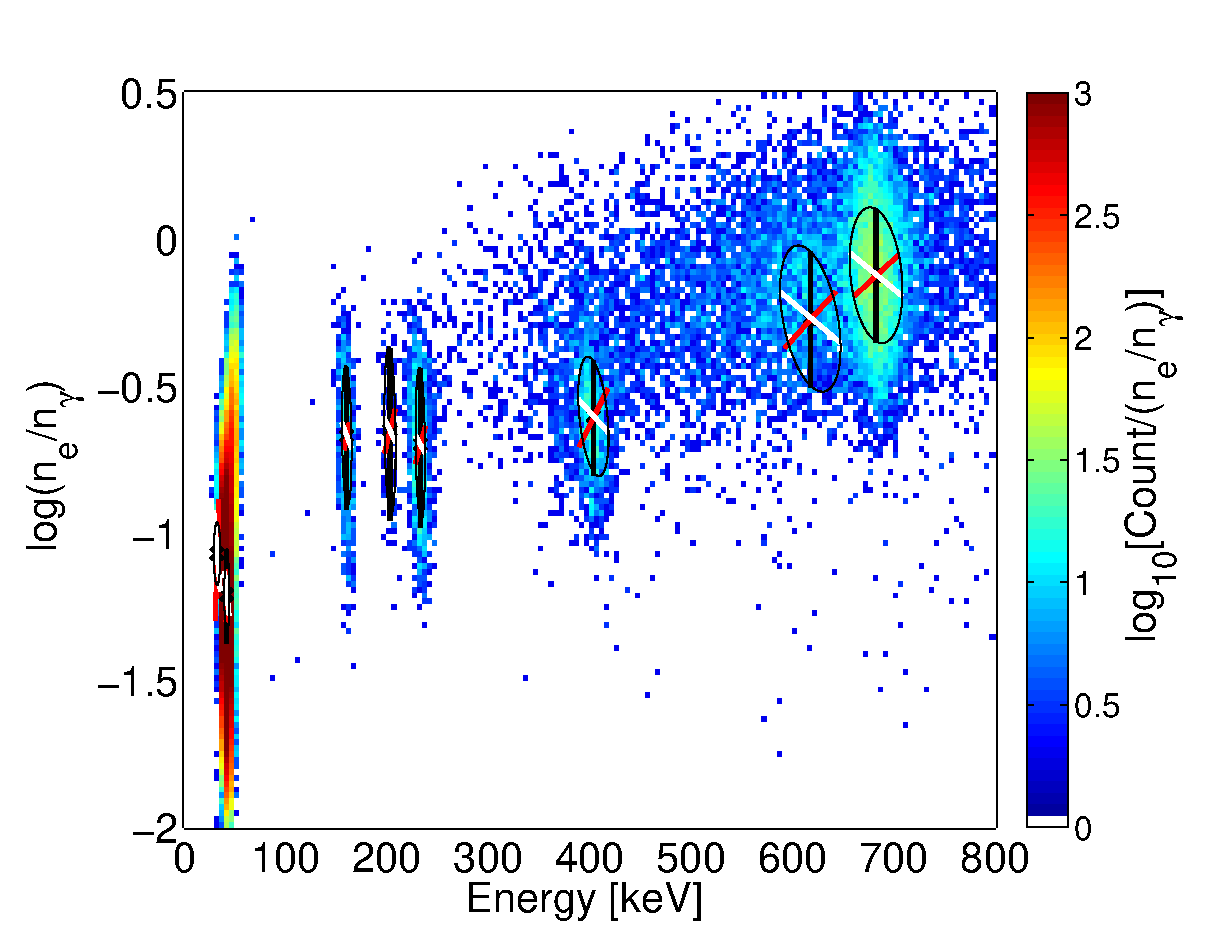
\includegraphics[width=120mm]{Chapter_Flucs/Figures/All_disc.eps}
\caption{Populations of calibration sources in discrimination space $\rm log\left(\frac{n_e}{n_\gamma}\right) $ vs. combined energy [$\rm keV_{ee}$]. The ovals represent the combination of $\rm \sigma R, \, \sigma n_{\gamma_{Det}}, \,\sigma n_{e_{Det}} $ in black, white, red respectively.}
\label{fig:E_dis}
\end{figure}

 \begin{figure}[h!]\centering
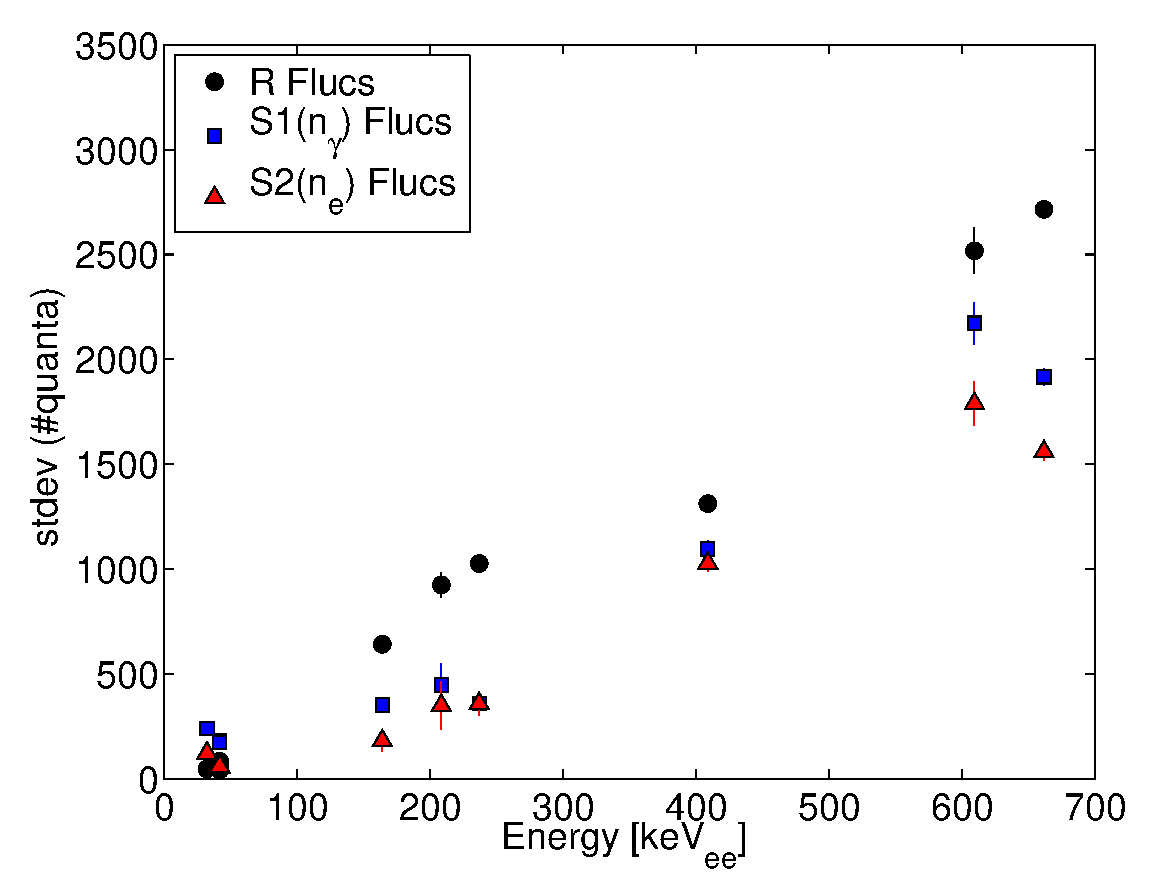
\includegraphics[width=70mm]{Chapter_Flucs/Figures/fluc_E.eps}
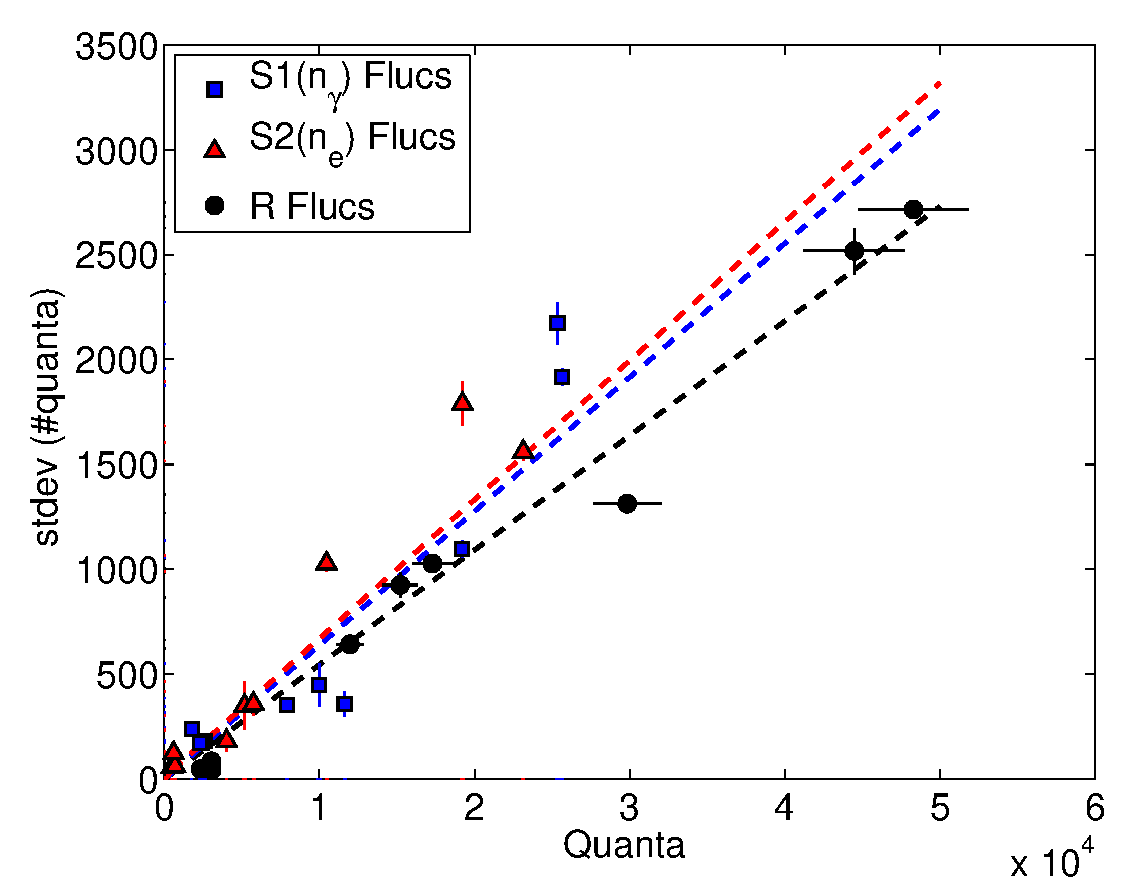
\includegraphics[width=70mm]{Chapter_Flucs/Figures/fluc_Q.eps}
\caption{Measured values of $\rm \sigma R, \, \sigma n_{\gamma_{Det}}, \,\sigma n_{e_{Det}} $ vs. Energy on the left and vs. Quanta on the right. Measured using sources listed in Table \ref{table:Cal_lines}. }
\label{fig:Flucs}
\end{figure}


\section{Measuring Recombination Fluctuations in Desecrate Energy Bins}
\label{sec:flucs_mono_bins}

The pervious subsection demonstrated the power of using a mono energetic source measure recombination fluctuations, equation  \ref{eq:Dahl}. In this section we present a method to decouple statistical variance from recombination fluctuations when confined to an energy bin of width $\rm \Delta_E$. The consideration of desecrate binning is crucial when dealing with a continual energy spectrum. Take the tritium beta spectrum as an example, we lose the ability to independently measure $\rm \sigma_{n_\gamma}^2$, $\rm \sigma_{n_e}^2$, $\rm \sigma_{E}^2 $ and are only left with a smear of $\rm n_\gamma$, $\rm n_e$, $\rm E $. However, there are two key pieces of information still left at our disposal. First, the combined energy can be reconstructed from global fits to g1 and g2, and even corrected for spectral shape and detector resolution (discussed later in section [link]). Second, we can calculate values of statistical variance for the light and charge channels as a function of energy, described in \ref{eq:SigStat},  \ref{eq:SigInst}. It will be shown in this section that having a priori knowledge of g1 and g2 and the functional for of the statistical variance from detector resolution will be sufficient to measure recombination fluctuations for a continual energy spectrum binned in energy with width $\rm \Delta_E$.


We begin the treatment of binning with the the case of having a finite bin width around the central combined energy of a mono energetic source. First, we quantify the change in the statistical components of equation \ref{eq:SigR} when slicing out a bin in combined energy space. The slice in combined energy is illustrated for a toy model at quanta corresponding to that of the combined 41.6 keV $\rm^{83}Kr$ decay in Figure \ref{fig:Recomb}. All contribution from recombination fluctuations are included when slicing out a section of combined energy, illustrated in Figure \ref{fig:Recomb}. However, the slice contains only a reduced statistical component from both the light and charge signals, and in the limit that $\rm \Delta E$ goes to zero the statistical component of light and charge converge to a value defined as $\rm \chi_{stat}$ (where $\rm \chi$ is the measured $\rm \sigma$ in a bin of combined energy). To solve for the value of  $\rm \chi_{stat}$ we first calculate the slope induced by statistical variance in the number of photons vs. quanta and the complementary slope of electrons vs. quanta, defined as M and 1-M respectively.  The value of M depends on the magnitude of the statistical variances and is given in equation \ref{eq:Angle}. The sum of the two slopes must equal one as the sum of photons and electors make up combined energy.


 \begin{figure}[h!]\centering
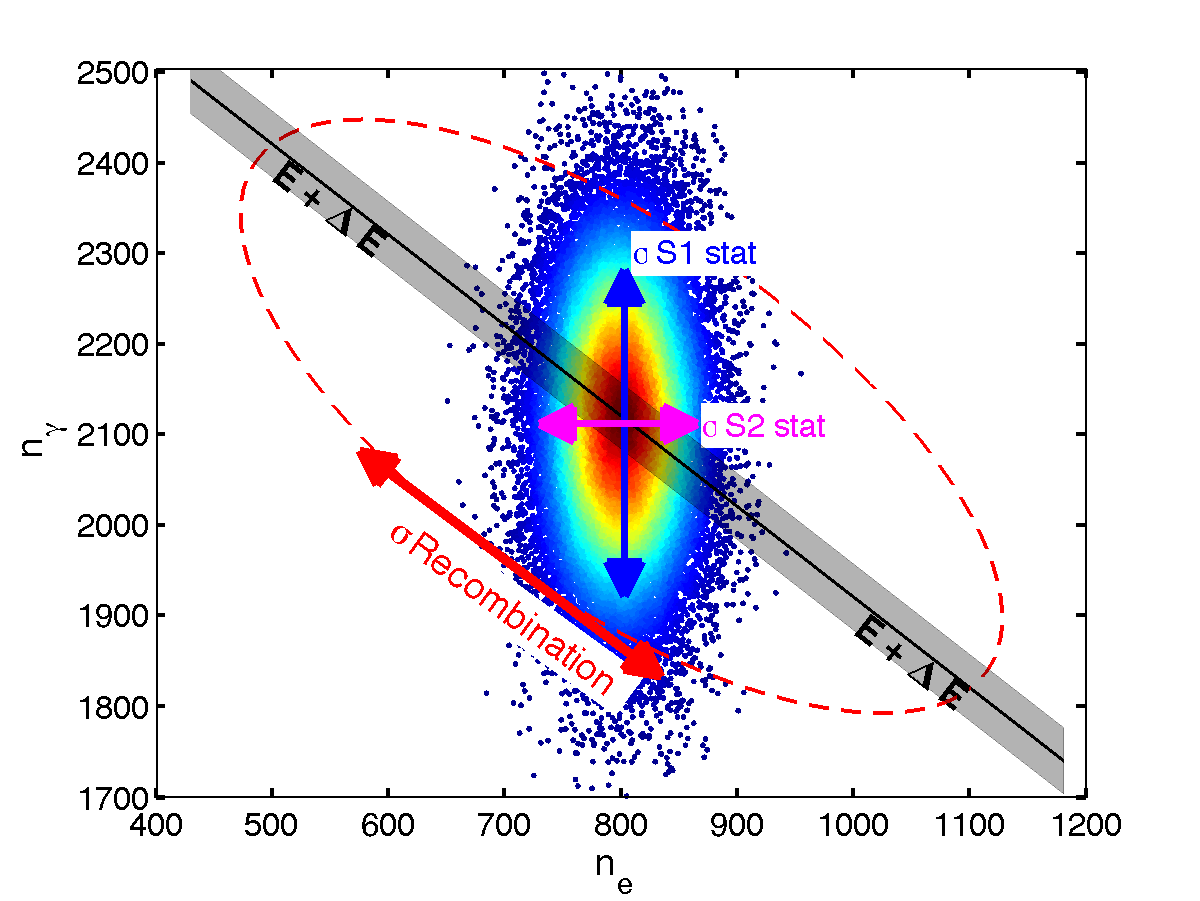
\includegraphics[width=130mm]{Chapter_Flucs/Figures/EX_Stat_Fano.png}
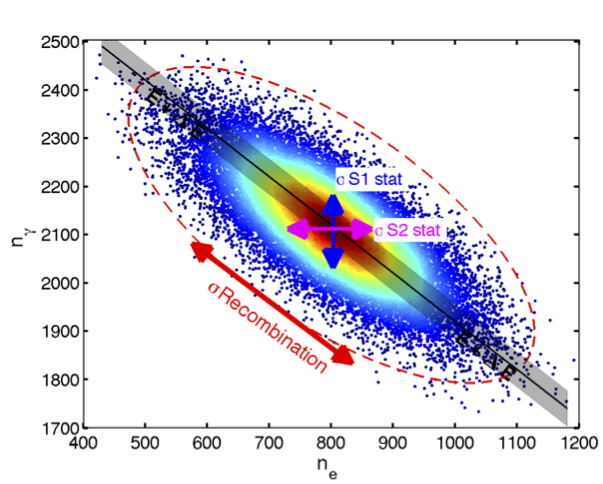
\includegraphics[width=60mm]{Chapter_Flucs/Figures/EX_R_Fano.png}
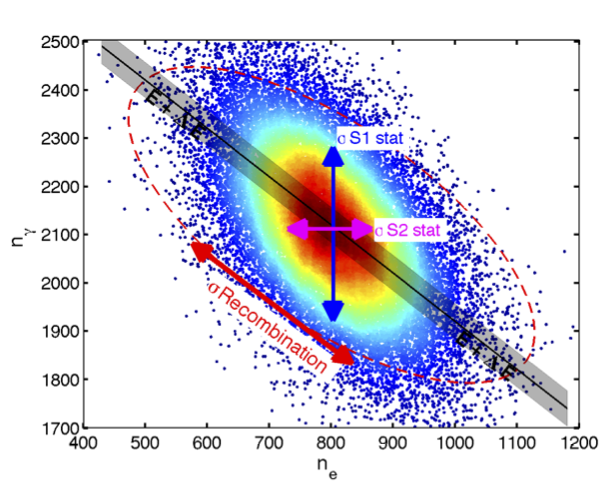
\includegraphics[width=60mm]{Chapter_Flucs/Figures/EX_Kr_Fano.png}
\caption{Top: Illustration of statistical variance, recombination fluctuations are set to 0. The spread in number of photons moves vertically and the spread in number of electrons moves horizontally. In black, a line of constant energy along the mean of combined energy with a width $\rm \Delta E$. Bottom left: Dominated by recombination fluctuations which move 45$^{\circ}$ to statistical variances. Bottom Right: Typical values for recombination and  S1, S2 Stat for $\rm Kr^{83}$. }
\label{fig:Recomb}
\end{figure}

\begin{equation}
\begin{split}
\rm M = tan(\theta_{n_{\gamma_{Det}}})=\frac{\sigma_{n_{\gamma_{Det}}}^2}{\sigma_{n_{\gamma_{Det}}}^2+ \sigma_{n_{\gamma_{Det}}}^2} \\
\rm 1-M = tan(\theta_{n_{e_{Det}}})=\frac{\sigma_{n_{e_{Det}}}^2}{\sigma_{n_{\gamma_{Det}}}^2+ \sigma_{n_{\gamma_{Det}}}^2} 
\label{eq:Angle}
\end{split}
\end{equation}


With the slope between combined energy and $\rm \sigma_{n_{\gamma_{Det}}}$ and between energy and $\rm \sigma_{n_{e_{Det}}}$ defined in equation \ref{eq:Angle} the value of the shared statistical uncertainty in combined energy space can be determined. We first treat the case of $\rm \Delta E$ = 0 in equation \ref{eq:SigCE} which is also valid when the centroid of light yield and change yield has been subtracted (discussed later).

\begin{equation}
\rm \chi_{Det}^2= M^2\sigma_{n_{e_{Det}}}^2 + (1-M)^2\sigma_{n_{\gamma_{Det}}}^2
\label{eq:SigCE}
\end{equation}


The variable $\rm \chi$ is used to represent the observed $\rm \sigma$ when dealing in bins of combined energy. Let's briefly consider the implication of equation \ref{eq:SigCE}. For the case of $\rm \sigma_{n_{e_{Det}}}^2 = \sigma_{n_{\gamma_{Det}}}^2$, M=0.5, resulting in $\rm \sigma_{n_{e_{Det}}}^2=\sigma_{n_{\gamma_{Det}}}^2= \chi_{Det}^2$. This case can be thought of as sweeping out equal variance from the statistical population which would for a circle as illustrated in Figure \ref{fig:Recomb}. For the case of $\rm \sigma_{n_{e_{Det}}}^2 \neq \sigma_{n_{\gamma_{Det}}}^2$ the observed statistical variance in a slice of combined energy will become less than the variance of the best channel. Specifically for the LUX detector the implication of equation \ref{eq:SigCE} is that the statistical variance measured in a slice of combined energy will collapse to less than that of the S2 statistical uncertainty, as bin width $\rm \Delta_E$ goes to zero.


To complete the treatment of binned energy in this section we now add the final piece to the observed statistical variance, the contribution from the bin width $\rm \Delta_E$. The residual variance arrises from rotating the population of 2D gaussian about the bin center, the rotation having a slope of M or (1-M) as given in equation \ref{eq:Angle}. Note, the residual term from the slope can also be removed by centroid subtraction of the photons and electrons vs. energy as discussed later in section \ref{sec:Centroid}, in that case we are only left with $\chi_{Det}^2$ shared between the two channels.


\begin{equation}
\begin{split}
\rm \chi_{n_{\gamma_{Det}}}^2= \chi_{Det}^2 + \frac{(MW\Delta_E)^2}{12}\\
\rm \chi_{n_{e_{Det}}}^2= \chi_{Det}^2 + \frac{((1-M)W\Delta_E)^2}{12}\\
\label{eq:SigCE_2}
\end{split}
\end{equation}



Were $\chi^2$ is defined in \ref{eq:SigCE}, M is given in equation \ref{eq:Angle}, W is the work function in [quanta/keV], $\rm \Delta_E$ is a bin of energy [keV], the normalization of 12 arrises from the second moment of a rotated line about its center. The total observed variance, $\rm \chi^2$, in the number of photons and electrons considering a bin of combined energy can now be determined transforming equation \ref{eq:SigR} to \ref{eq:Sig_total_CE}.

%%.... this equation holds for the standard deviation of a uniform distribution
 
\begin{equation}
\begin{split}
\rm \chi_{n_\gamma}^2 = \sigma_{n_{ex}}^2 + n_iF(r)^2 + \sigma_{r}^2 n_i^2 + \chi_{n_{\gamma_{Det}}}^2 \\
\rm \chi_{n_e}^2  = n_iF(1-r)^2 + \sigma_{r}^2 n_i^2 + \chi_{n_{e_{Det}}}^2
\label{eq:Sig_total_CE}
\end{split}
\end{equation}


In equation \ref{eq:Sig_total_CE} we have defined the observed standard deviation in units of quanta $\rm \chi$ for $\rm n_\gamma, n_e$ when working with bins of combined energy. In the limit that F, $\rm \sigma_{n_{ex}}^2$ and $\rm \Delta_E$ go to zero the observed variance in number of photons and electrons ($\rm \chi_{n_\gamma}$ and $\rm \chi_{n_e}$) are related to the size of recombination fluctuations in a given combined energy bin, equation \ref{eq:SigR_CE_lim}. Where $\rm \sigma R$ is in units of quanta, $\rm \sigma_R = n_i\sigma_r$.

\begin{equation}
\begin{split}
\rm \sigma_{R_\gamma}^2 = \chi_{n_\gamma}^2 - \chi_{n_{\gamma_{Det}}}^2  \\
\rm \sigma_{R_e}^2 = \chi_{n_e}^2 - \chi_{n_{e_{Det}}}^2
\label{eq:SigR_CE_lim}
\end{split}
\end{equation}

We have arrived at the conclusion of this section, armed with equation \ref{eq:SigR_CE_lim} we now have two methods for determining the size of recombination fluctuations, $\rm\sigma_{R}^2$ where the subscript $\rm \gamma$ or e is used to represent the channel of quanta used for the calculation. Either the observed variance in the light and charge channel can be used to measure the size of recombination fluctuation in a bin of energy. Any asymmetry between the two methods has implications which are discussed in the following subsection.


\subsection{Measuring the Fano Factor in Bins of Energy}

There are three terms in equation \ref{eq:Sig_total_CE} that give rise to an asymmetry between the observed variance $\rm \sigma_{R_\gamma}^2$  and  $\rm \sigma_{R_e}^2$. The small difference in variance from the slope can be solved for exactly leaving just the Fano factor F and $\rm \sigma_{n_{ex}}^2$. By taking the difference of variance in the two channels component of recombination variance drops out leaving only the Fano factor and the variance in number of excitons, given in equation \ref{eq:Sig_total_CE}.

\begin{equation}
\rm \sigma_{R_\gamma}^2 - \sigma_{R_e}^2 = \sigma_{n_{ex}}^2 + n_iF(2r-1) 
\label{eq:Diff_X}
\end{equation}

F is the Fano factor, equation \ref{eq:Energy_2}, $\rm \sigma_{n_{ex}}^2$ is the variance of the number of excitons produced and r is the recombination fraction, equation \ref{eq:Quanta}. %The value of $\delta_{Det}$ is the small residual depending on the bin width $\rm \Delta_E$, equation \ref{eq:Residual_Stat}.
%\begin{equation}
%\rm \delta_{Det}= \sigma_{R_\gamma}^2 - \sigma_{R_e}^2 = \frac{(1-2M)(W\Delta_E)^2}{12}\\
%\label{eq:Residual_Stat}
%\end{equation}
Consider the case such that variance in the number of excitons $\rm \sigma_{n_{ex}}^2$ is much less than the contribution from the Fano factor. In such a regime we can solve for the Fano factor, potentially energy dependent, from equations \ref{eq:Diff_X}.

\begin{equation}
\rm F(E)=\frac{\sigma_{R_\gamma}^2 - \sigma_{R_e}^2}{n_i(2r-1)}
\begin{cases} \rm r \neq \frac{1}{2}\\
\end{cases}
\label{eq:Fano}
\end{equation}

There is an underlying subtlety to equation \ref{eq:Fano}. Remarkably, in the limit that $\rm \Delta_E$ goes to zero the Fano factor can be extracted with minimal knowledge of intrinsic detector statistical variance. Further, when the statistical variance of S1 and S2 are identical the value of M (equation \ref{eq:Residual_Stat}) will be 0.5. In that special case no knowledge of the statistical variance is needed to measure the Fano factor. 


When $ \rm r = \frac{1}{2}$ the coefficient in front of the Fano factor becomes zero in equation \ref{eq:Diff_X}. At this value an equal contribution from the Fano factor goes into the variance $\rm \chi^2$ of photons and electrons, allowing for the smaller value of $\rm \sigma_{ex}^2$ to be extracted. 

\begin{equation}
\rm \sigma_{n_{ex}}^2=\sigma_{R_\gamma}^2 - \sigma_{R_e}^2
\begin{cases} \rm r= \frac{1}{2} || \sigma_{n_{ex}}^2 > > n_iF(2r-1)\\
\end{cases}
\label{eq:SigmaEx}
\end{equation}

Equation \ref{eq:SigmaEx} is also valid in the case that $\rm \sigma_{n_{ex}}^2$ is much larger than the contribution form the Fano factor. This happens to be true when dealing with the time dependent light yield of $\rm ^{83m}Kr$, this topic will be explored in the next section.




\subsection{Application to $\rm^{83}Kr$}

Using the high stats Kr83 calibration data we can validate the method for working in a bin of energy since the exact solution for recombination and detector fluctuations can be measured, as outlined in section \ref{sec:flucs_mono} and \ref{sec:flucs_mono_bins}. Once the fluctuations from detector resolution are measured in the light and charge channel (S1 and S2 signals), the asymmetry between the two channels can be used to calculate the Fano factor (equation \ref{eq:Sig_total_CE} ). The asymmetry in fluctuations in the light and charge channel arrises from the Fano factor acting on ion production which is later amplified through the recombination fraction, as long as the recombination fraction does not equal 0.5. For the case of the $\rm ^{83m}Kr$ calibration the recombination fraction was 0.772 resulting in recombination fluctuations of 3 to 4 more quanta in the light channel as compared to the charge channel, see table \ref{table:R_Kr}. Though the additional recombination fluctuation is small having ample statistics the Fano factor can be constrained. 
The errors in the measurement were derived from simulated Kr data sets of 400,000 events with the Fano factor turned off, using 100 trials. First, recombination fluctuations were turned off and only fluctuations from detector resolution as calculated in section \ref{sec:flucs_mono} were used, see Table \ref{table:Simulated_Sigmas_R_0}. It was found that the error of the difference in recombination fluctuation from the light and charge channel ($\rm sigma_{R_{\gamma}}^2$ and $\sigma_{R_{e}}^2 $) along with the error in ion production and recombination fraction were enough to constrain the Fano factor to 0.001-0.003. Next, the value of recombination was set slightly higher than the actual value of 82 to 100 quanta and the trials were repeated, see table \ref{table:Simulated_Sigmas_R_100}. With the addition of recombination fluctuations to detector resolution fluctuations the error on measuring the Fano factor grew to 0.002-0.009, with smaller bin sizes ($\rm\Delta E$ around the center leading to the smallest error as seen from equation \ref{eq:SigCE_2}.


\begin{table}[h!]
\begin{center}
\begin{tabular}{|c|c|c|c|c|c|}
\hline
$\rm \Delta_E$ [keV] & Count & $\rm \sigma (\sigma_{R_{\gamma}}^2 ) $ & $\rm \sigma (\sigma_{R_{e}}^2 )$  & $\rm \sigma (\sigma_{R_{\gamma}}^2 - \sigma_{R_{e}}^2 ) $ & $\rm \sigma F$ \\ \hline
0.025 	& 1528 		&77.8		& 77.9	  	& 1.3	&	0.0008 \\ \hline
0.05 	& 3063 		&54.4		& 54.6	  	& 1.8	&	0.0012 \\ \hline
0.1 		& 6128  	&36.4		& 36.6		& 2.6	&	0.0016  \\ \hline
0.2 		& 12242  	&23.7		& 23.8	 	& 3.7	&	0.0023 \\ \hline
0.25 	& 15290 	&22.9		& 22.9		& 4.0 	&	0.0026 \\ \hline
0.5		& 30528 	&17.5		& 17.5 		& 5.2	& 	0.0033	 \\ \hline
\end{tabular}
\caption{Values for the standard deviation of the observed value of $\rm \sigma_R^2$ from $\rm n_\gamma$ and $\rm n_e$ along with the standard deviation of the difference, for a simulated $\rm^{83m}Kr$ decay with recombination set to zero.  Note, since the two methods for determining $\rm \sigma_R^2$  are correlated the standard deviation of the measured difference is small leading to an improved error when calculating the Fano factor or $\rm \sigma_{n_{ex}}^2$.}
\label{table:Simulated_Sigmas_R_0}
\end{center}
\end{table}

\begin{table}[h!]
\begin{center}
\tabcolsep=0.11cm
\begin{tabular}{|c|c|c|c|c|c|}
\hline
$\rm \Delta_E$ [keV] & Count & $\rm \sigma (\sigma_{R_{\gamma}}^2 ) $ & $\rm \sigma (\sigma_{R_{e}}^2 )$  & $\rm \sigma (\sigma_{R_{\gamma}}^2 - \sigma_{R_{e}}^2 ) $ & $\rm \sigma F$ \\ \hline
0.025 	& 1523		&498		& 498	  	& 3.2	&	 0.0020\\ \hline
0.05 	& 3056 		&347		& 347	  	& 4.1	&	 0.0026\\ \hline
0.1 		& 6118  	&237		& 237		& 5.3	&	 0.0033\\ \hline
0.2 		& 12225  	&171		& 171	 	& 8.6	&	 0.0054\\ \hline
0.25 	& 15285 	&149		& 148		& 9.5 	&	 0.0060\\ \hline
0.5		& 30514 	&101		& 99.4  		&14.3	&	 0.0090 \\ \hline
\end{tabular}
\caption{Values for the standard deviation of the observed value of $\rm \sigma_R^2$ from $\rm n_\gamma$ and $\rm n_e$ along with the standard deviation of the difference, for a simulated $\rm^{83m}Kr$ decay with recombination set to 100 quanta.  Note, since the two methods for determining $\rm \sigma_R^2$  are correlated the standard deviation of the measured difference is small leading to an improved error when calculating the Fano factor or $\rm \sigma_{n_{ex}}^2$.}
\label{table:Simulated_Sigmas_R_100}
\end{center}
\end{table}


The results of the high stats calibration data are shown in table \ref{table:R_Kr}, containing 400k events in the fiducial volume of the detector. Using equation \ref{eq:SigR_CE_lim} we find good agreement between the method described in equation \ref{eq:Dahl} and the recombination fluctuation calculated from the charge channel ($\rm \sigma_{R_\gamma}$ and $\rm \sigma_{R_e}$).  The accuracy helps us build confidence that the statistical components of the detector are modeled well enough to measure recombination fluctuation to within 3\%. Further, the ability to see the asymmetry in recombination fluctuations between the light and charge channel demonstrates the power of using binned combined energy (section \ref{sec:flucs_mono_bins}). Any observed difference between the two channels  can only be from either the Fano factor or spread in exiton production, but we assume the fluctuations in exiton production are much less than fluctuations in ion production. The Fano factor is derived from equations \ref{eq:Fano} and the uncertainty was determined from simulations. The total fluctuation as number of quanta is listed in the rightmost column. The Fano factor manifests itself as an asymmetry between fluctuations in the light and charge channel as given in equation \ref{eq:Sig_total_CE}, the recombination fraction was found to be r= 0.772 and the average number of ions produced per decay was $\rm n_i=2900$. 
Having demonstrated the method for a mono energetic calibration source the next step will be to apply the method on the continuous beta spectrum of the tritium data.



\begin{table}[h!]
\begin{center}
\footnotesize
\tabcolsep=0.11cm
\begin{tabular}{|c||c|c|c|c|c|c|}
\hline
$\rm \sigma_R$ \ref{eq:Dahl} & $\rm \Delta_E$ & Count & $\rm \sigma_{R_\gamma}=\sqrt{\chi_{n_{\gamma}}^2-\chi_{n_{\gamma_{Det}}}^2}$ & $\rm \sigma_{R_e}= \sqrt{\chi_{n_{e}}^2-\chi_{n_{e_{Det}}}^2}$  & $\rm F=\frac{\sigma_{R_{\gamma}}^2-\sigma_{R_e}^2}{n_i(2r-1) }$ &$\rm \sqrt{Fn_i}$ \\ 
(Quanta) & (keV) & & (Quanta) & (Quanta) & (Quanta) & (Quanta)\\ \hline
82.4 $\pm$ 4.0		& 0.025		& 1518 		& 87.2 $\pm$ 2.9	 	&	87.1 $\pm$ 2.9	& 0.010 $\pm$ 0.002     & 5.8 $\pm$ 0.5 \\ \hline
					& 0.05 		& 3124 		& 85.0 $\pm$ 2.0	 	&	84.9 $\pm$ 2.0	& 0.005 $\pm$ 0.003	& 3.8 $\pm$ 1.1 \\ \hline
					& 0.1 		& 6269  	& 87.8 $\pm$ 1.3		& 	87.6 $\pm$ 1.3	& 0.023 $\pm$ 0.003	& 8.1 $\pm$ 0.5	 \\ \hline
					& 0.2 		&12508  	& 90.0 $\pm$ 1.0  		& 	89.7 $\pm$ 1.0	& 0.021 $\pm$ 0.005	& 7.8 $\pm$ 0.9	 \\ \hline
					& 0.25 		&15557 	& 88.5 $\pm$ 0.8		&	88.3 $\pm$ 0.8  & 0.013 $\pm$ 0.006	& 6.1 $\pm$ 1.3	 \\ \hline
					& 0.5		& 30826 	& 87.0  $\pm$ 0.6		&	86.7 $\pm$ 0.6	& 0.027	$\pm$  0.009 	& 8.8 $\pm$ 2.2	\\ \hline
\end{tabular}
\caption{Values for the standard deviation of the observed value of $\rm \sigma_R^2$ from $\rm n_\gamma$ and $\rm n_e$ along with the standard deviation of the difference, for a $\rm^{83m}Kr$ data set with 400k events in the fiducial volume. The Fano factor is derived from equations \ref{eq:Fano} and the uncertainty was determined from simulations. The total fluctuation as number of quanta is listed in the rightmost column. The Fano factor manifests itself as an asymmetry between fluctuations in the light and charge channel as given in equation \ref{eq:Sig_total_CE}, with a recombination fraction of 0.772 and $\rm n_i = 2900$. }% add note about excitons
\label{table:R_Kr}
\end{center}
\end{table}


\subsection{Application to Simulated Tritium Data (any continuous spectrum)}

%ref Partrick
%This will be demonstrated later (or maybe show it in the simulation)
Adapting the equation of the previous section to continuous energy spectra requires that the centriod of a continue spectrum be subtracted off so that the variance from the light yield or charge yield vs. energy is removed. After applying the Smearing Model of Section 4 we apply the method described in this section to extract recombination fluctuations form the tritium data.

In this subsection we test method outlined in section \ref{sec:flucs_mono_bins} for dealing in bins of combined energy specifically applied to the tritium beta spectrum, but the method outlined can be used for any continue spectrum. To first order the treatment of the continuous spectrum is identical to that outlined for the mono energetic source as outlined previously in subsection \ref{sec:flucs_mono_bins}. Figure \ref{fig:T_Stat} illustrates a tritium beta spectrum convolved with detector resolution similar to that measured for the LUX detector, the figure is analogous to Figure \ref{fig:Recomb}. As the bin size around a value of combined energy is squeezed to zero the statistical variance in the number of photons and electrons converge, the value is given by equation \ref{eq:SigCE_2}. Whereas, regardless of bin size recombination fluctuations remain since they move along lines of constant energy. In order to adapt the methodology developed for a mono energetic source to a continuous energy spectra requires that the centriod of the light and charge yield be subtracted off. The slope in the light and charge channels from the fundamental yield  induce a further variance on top of $\rm \chi_{Det}$ from the population in an energy bin being tilted as demonstrated in figure \ref{fig:SIM_LYQY}. For the purposes of this study, we find it sufficient to fit a quadratic form to the centroid of the entire population and subtract off the local slope from the measured variance. An analogous methods for centriod subtraction to extract recombination fluctuations are described in detail in [Patrick's Thesis].



\begin{figure}[h!]\centering
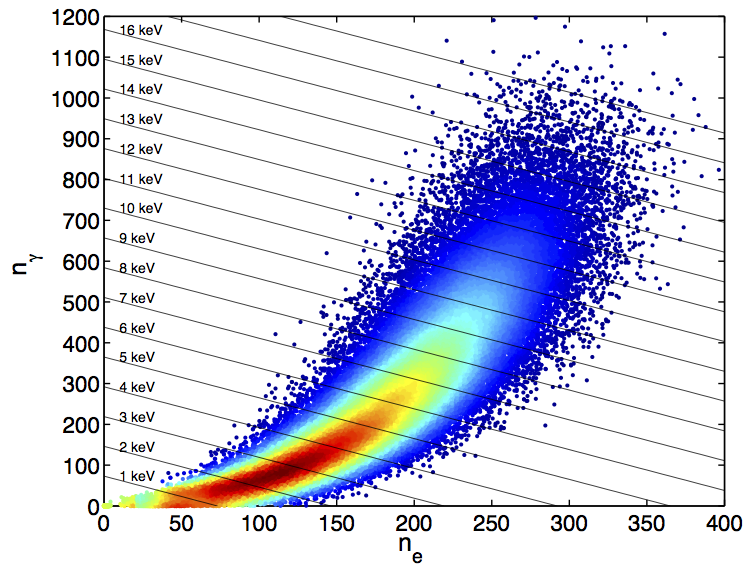
\includegraphics[width=130mm]{Chapter_Flucs/Figures/EX_T_Fano.png}
\caption{Illustration of statistical variance for the tritium beta spectrum, recombination fluctuations are set to 0. This plot is analogous to Figure \ref{fig:Recomb} which illustrates the case for the mono energetic $\rm ^{83m}Kr$ decay. Recombination fluctuation move along lines of constant energy, S1 statistical fluctuation move vertically and S2 statistical fluctuations move horizontally. }
\label{fig:T_Stat}
\end{figure}

\begin{figure}[h!]\centering
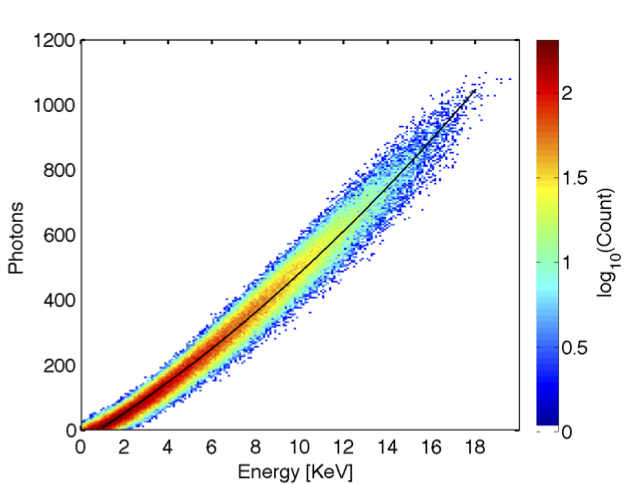
\includegraphics[width=70mm]{Chapter_Flucs/Figures/T_SIM/n_photon_180_.png}
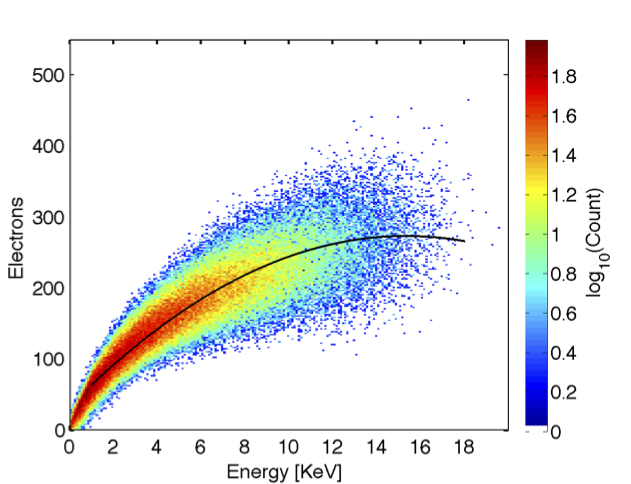
\includegraphics[width=70mm]{Chapter_Flucs/Figures/T_SIM/n_e_180_.png}
\caption{Light yield (left) and Charge yield (right) of a simulated tritium spectrum, with the fit to the centroid show in black. The variance in number of photon and electrons per energy bin is used to extract recombination fluctuations.}
\label{fig:SIM_LYQY}
\end{figure}

%Add centriod subtracted equation. Explain that even if S1, S2 Det are off we can do as good as the best channel (S2) due to X_Det. As long as SigR is greater, since they add in quadrature.


\subsection{Centriod Subtraction}
\label{sec:Centroid}
For the case of a continuous source we expand upon the result from section \ref{sec:flucs_mono_bins} where the additional variance from detector resolution was calculated per energy bin as $\rm \chi_{n_{\gamma_{Det}}}^2$ and $\rm \chi_{n_{e_{Det}}}^2$. When dealing with a continuous source we must subtract off the centroid of the number of photons and electron vs. energy to remove additional variance induced by the slope. What results is a common variance from detector resolution shared by both the charge and light channel in each bin of energy, defined as $\rm \chi_{Det}^2$ = $\rm \chi_{n_{\gamma_{Det}}}^2$ = $\rm \chi_{n_{e_{Det}}}^2$, equation \ref{eq:SigR_Cent}. The value of $\rm \chi_{Det}^2$ is derived in \ref{eq:Centroid} for a small variation in $\rm n_e$ around combined energy, and is identical to that found for the case of the mono energetic source in equation \ref{eq:SigCE}. This is analogous to saying that the centroid subtraction is removing the additional variance from the slope of light field and charge yield. The local slope of  $\rm n_e$ with respect to quanta ($\rm n_\gamma + n_e$) is (1-M), given in \ref{eq:Angle}. 
To demonstrate the effectiveness of the method we use the measured detector resolution along with a test recombination fluctuation and simulate a tritium spectrum. The result of extracting recombination is shown in figure \ref{fig:T_Var} for various energy bin widths. As long as the recombination is greater than $\rm \chi_{Det}$, which is being added in quadrature, the value of recombination can be determined to good precision using the method. The small deviation around the first and last bins is due to the spectral shape, a correction for spectral shape will be discussed in the next section and will improve the measurement of $\rm \sigma_R$. The analytic solution for extracting recombination given in equation \ref{eq:SigR_Cent} is sufficient to first order, we ignore second order corrections in this analysis. After correcting observables for the tritium beta spectral shape we will be ready to use the tools of this section to decouple detector resolution and measure recombination fluctuations from the tritium data

\begin{equation}
\begin{split}
\rm \sigma_{R_\gamma}^2 = \chi_{n_\gamma}^2 - \chi_{Det}^2  \\
\rm \sigma_{R_e}^2 = \chi_{n_e}^2 - \chi_{Det}^2 \\
\label{eq:SigR_Cent}
\end{split}
\end{equation}


\begin{multline}\\
\delta[\Delta n_e] = \delta[n_e] - \delta\left[\left<n_e\right>_{n_e+n_\gamma}\right]  \\
= \cancelto{1}{\frac{dn_e}{dn_e}} \delta[n_e] + \cancelto{0}{\frac{dn_e}{dn_\gamma}} \delta[n_\gamma] - \delta \left[\left<n_e\right>_{n_e+n_\gamma}\right] \\
= \delta[n_e] - \frac{d \left<n_e\right> }{d(n_e+n_\gamma)} \frac{d(n_e+n_\gamma)}{dn_e} \delta[n_e] - \frac{d\left<n_e\right>}{d(n_e+n_\gamma)} \frac{d(n_e+n_\gamma)}{dn_\gamma} \delta[n_\gamma] \\
\delta[\Delta n_e] = \delta[n_e] - \left(\delta[n_\gamma] + \delta[n_e]\right) \frac{d\left<n_e+n_\gamma\right>}{d\left(n_e+n_\gamma\right)} \\
\delta[\Delta n_e] = (M)\delta[n_e] - (1-M) \delta[n_\gamma] \\
\chi_{Det}^2 = Var(\Delta n_e) = (M)^2\delta^2[n_e] + (1-M)^2\delta^2[n_\gamma]-2M(1-M) \cancelto{0}{\delta[n_e]\delta[n_\gamma]} \\
\label{eq:Centroid}
\end{multline}


\begin{figure}[h!]\centering
 
\subcaptionbox{\label{fig:1a}}{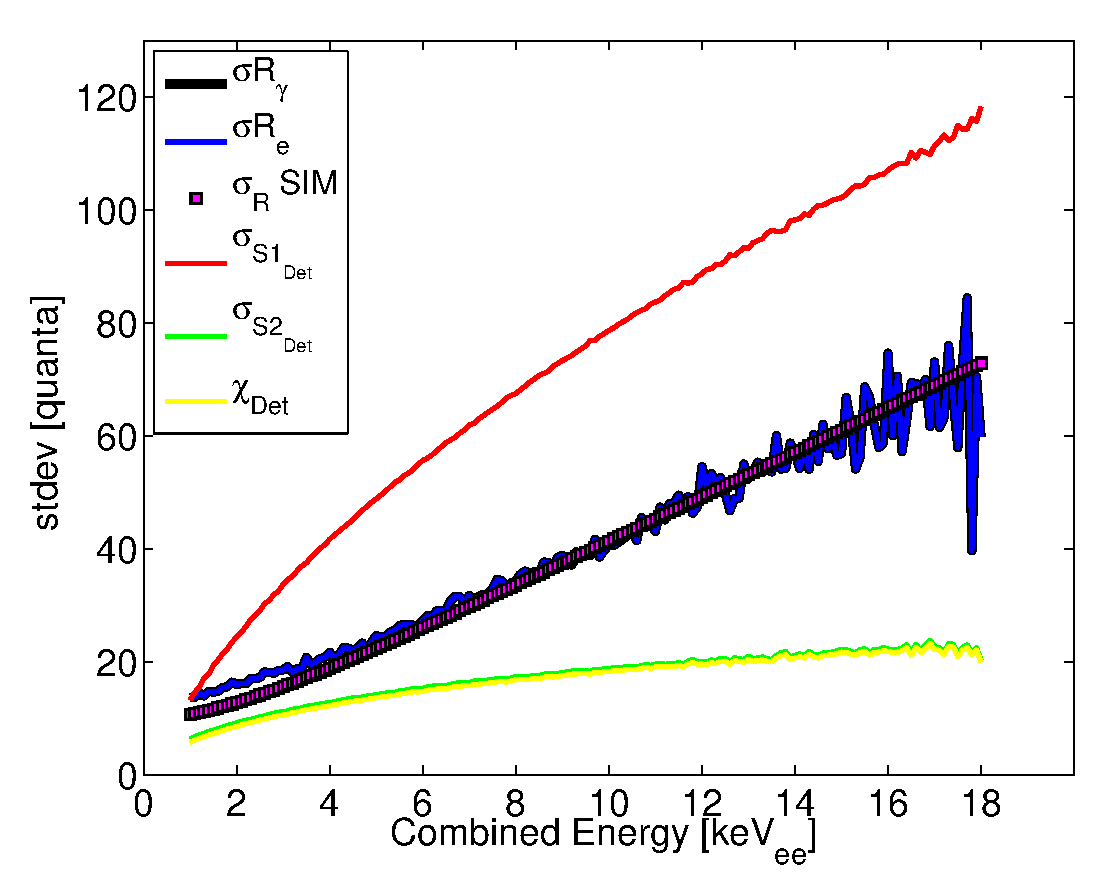
\includegraphics[width=70mm]{Chapter_Flucs/Figures/T_SIM/SIM_R_T_10.eps}}
\hfill
\subcaptionbox{\label{fig:1b}}{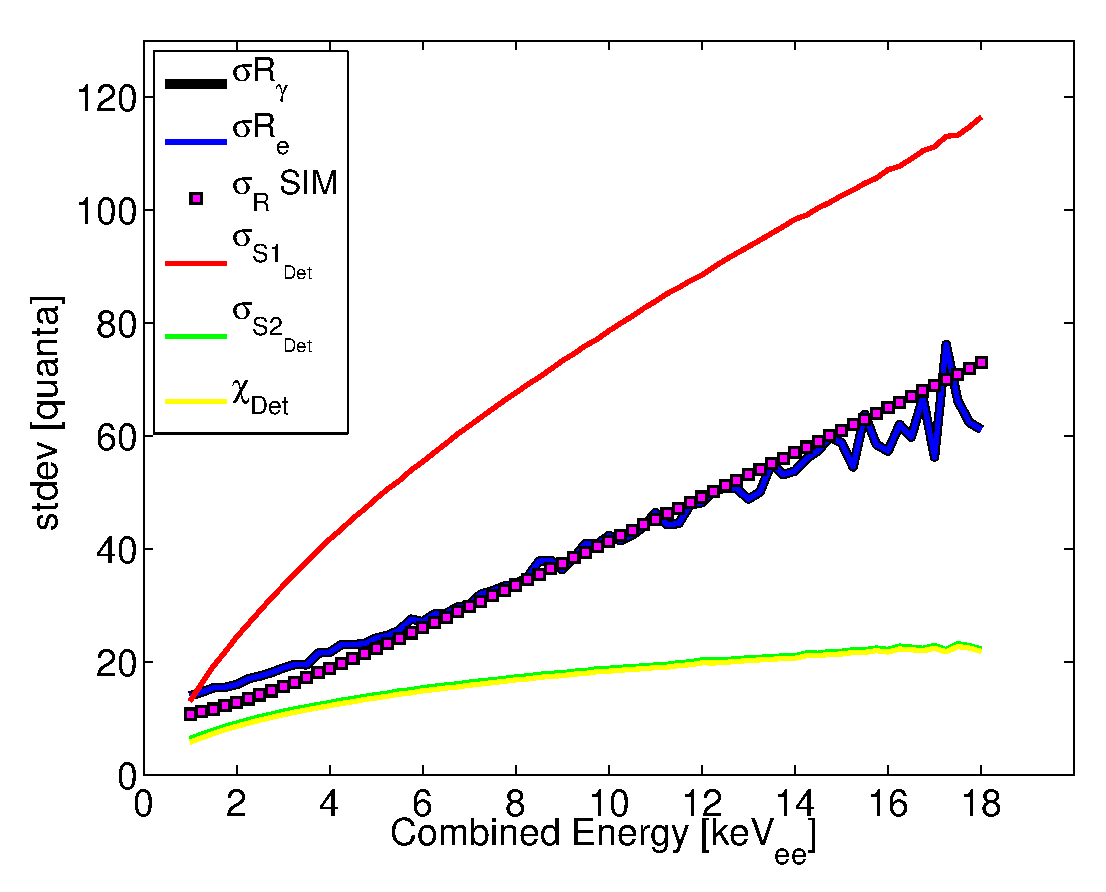
\includegraphics[width=70mm]{Chapter_Flucs/Figures/T_SIM/SIM_R_T_25.eps}}


\bigskip

\subcaptionbox{\label{fig:1c}}{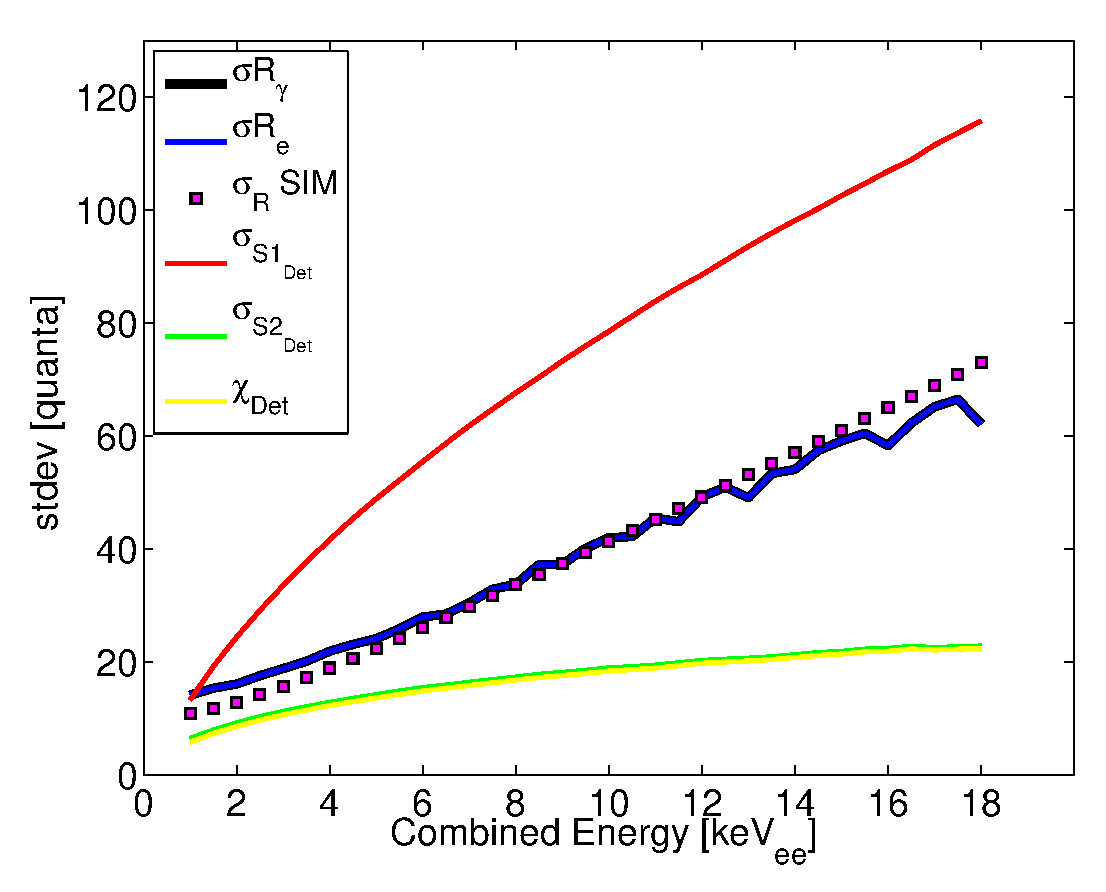
\includegraphics[width=70mm]{Chapter_Flucs/Figures/T_SIM/SIM_R_T_50.eps}}
\hfill
\subcaptionbox{\label{fig:1d}}{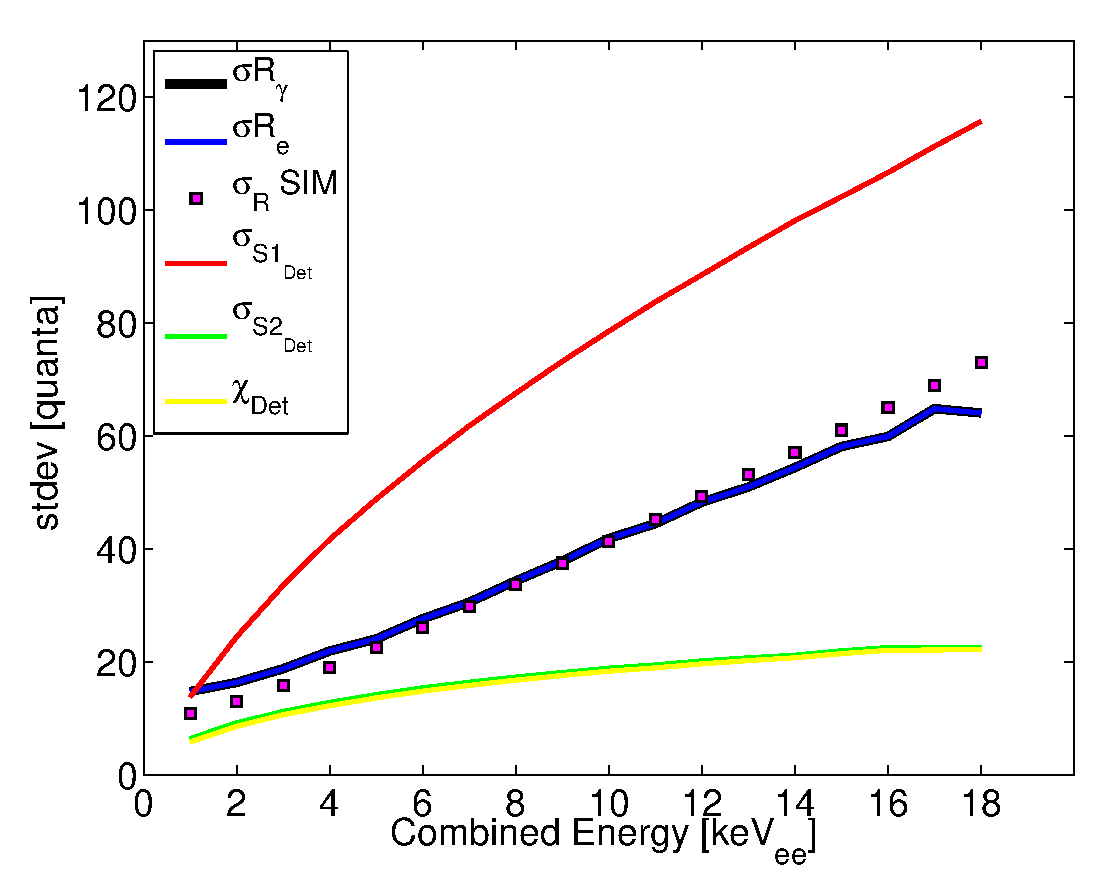
\includegraphics[width=70mm]{Chapter_Flucs/Figures/T_SIM/SIM_R_T_100.eps}}


\caption{Simulated tritium spectrum with the detector resolution of the LUX detector, $\rm \sigma_{S1_{Det}}$ and $\rm \sigma_{S2_{Det}}$, and an arbitrary recombination fluctuation $\rm \sigma R$ (magenta). After centroid subtraction we apply the methodology described in the previous section to extract $\rm \sigma R$ (black and blue) through the light and charge channel using our knowledge of detector resolution per each energy bin $\rm \chi_{Det}$ (green), $\rm S1_{Det}$ (red) and $\rm S2_{Det} $(yellow). The plots show cases for various bin widths in [KeV]: a) $\rm \Delta E$ = 0.1 b) $\rm \Delta E$ = 0.25 c) $\rm \Delta E$ = 0.5 d) $\rm \Delta E$ = 1.   }
\label{fig:T_Var}
\end{figure}% Extracting Recombination variance vs. delta E for a simulated tritium spectrum. The smaller deltaE the smaller the effect of slope on the measurement, though it is found that subtracting off the centroid with a quadratic fit is sufficient.


\newpage
\section{Correcting for Spectral Shape for Finite Resolution}
\label{sec:Smear}

%The goal of the following two sections is to extract light yield, charge yield and recombination fluctuations from the tritium spectrum using the methods described in section \ref{sec:flucs_mono_bins}. The first step is to use the NEST model in an attempt to undue the effect of the tritium spectral shape and finite detector resolution, described in this section. We find that the light yield and charge yields extracted from the data deviate too much to apply the correction factor. Since the correction is found to be small we can proceed to extract new LY, QY and $\rm \sigma R$ from the tritium data without correction building a model that better reproduces the data than the NEST model (which has yet to be vetted at our electric field and energy). We then take that improved model and apply the correction.
 
%The first step is to solve for the value of $\rm \sigma_R$ (recombination fluctuation) that needs to be input into the smearing model, the statistical part from detector resolution remains fixed. Figure \ref{fig:R_T} show the optimal value of $\rm \sigma_R$ being extracted from the tritium data, starting with an initial guess based on the recombination fluctuation measured from the $\rm^{83m}Kr$ data.

The distribution of tritium events convolved with the detector's finite resolution for S1 (scintillation) and S2 (ionization) causes the observed mean to shift from the actual mean. The shift is non trivial and depends on the spectral shape and the functional form resolution over a range of energies. A large negative derivative of the spectral shape will tend to pull the observed spectrum to lower values, and the functional form of the of resolution will also shift the spectrum. Figure \ref{fig:exp_int} and equations \ref{eq:2} and \ref{eq:4} demonstrate a simple model to solve for the relation between observed mean and actual mean. Take for example a linearly declining distribution, starting with infinite detector resolution we set up bins of width $\rm \Delta x$. To account for finite energy resolution we distribute the counts in each rectangular bin into Gaussians centered at $\rm \mu_i$, with a spread of $\sigma_i$, and normalized to the area of the bin $\rm N_i \times \Delta x $ with amplitude $\rm c_i$. Each rectangular bin(i) can be written as a Gaussian G(i): \\ 
\begin{multline}
\\ \rm c_i=\frac{N_i \times \Delta x}{\sigma_i\sqrt{2\pi}} \\
\rm G_{i}(x) = c_i \times exp\left(\frac{-(x-\mu_i)^2}{2\sigma_i^2}\right)\\
\label{eq:1}
\end{multline}


Where $\rm N_i$ is the count in the $\rm i^{th}$ bin, $\rm \Delta x$ is the bin width, $\rm \mu_i$ is the bin center and $\rm \sigma_i$ is the resolution at the $\rm i^{th}$ bin. Figure \ref{fig:exp_int} show the application of equation \ref{eq:1} to a linear energy distribution with a $\rm \sqrt{E}$ dependent $\sigma$. The observed distribution is the sum of the Gaussians, shown in red.

 \begin{figure}[h!]\centering
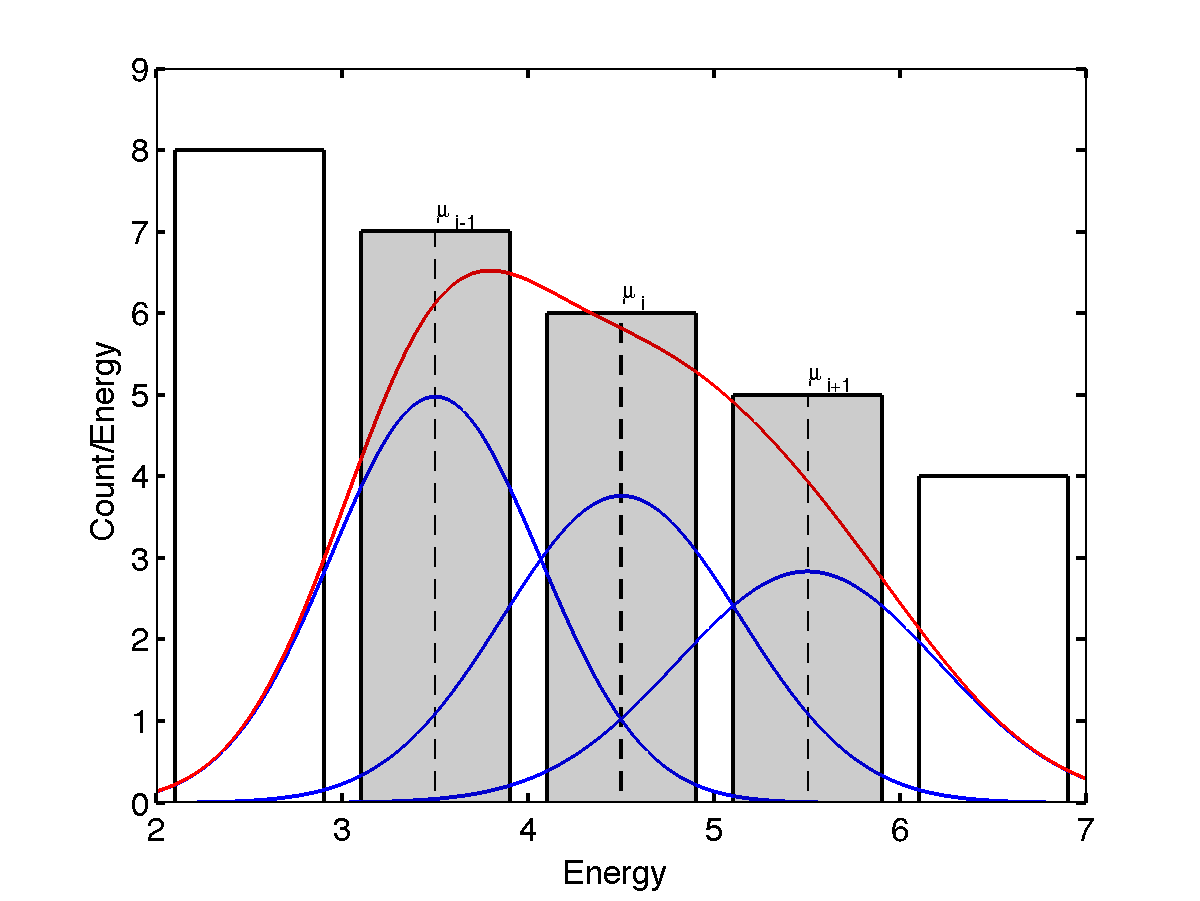
\includegraphics[width=130mm]{Chapter_Flucs/Figures/example_integral}
\caption{}
\label{fig:exp_int}
\end{figure}


\subsection{Calculating the Observed Energy}

After modeling the finite resolution with Gaussians the mean observed at each bin can be calculated from the overlap of all bins weighted by the corresponding means. We can write the observed mean in the $\rm i^{th}$ bin, $\nu_i$, in terms of the bin centers $\mu$ and overlapping areas of all bins using equation \ref{eq:1}:
%\begin{center}
\begin{equation}
\nu_i = \frac{\mathlarger{\sum}\limits_{j=1}^{n}\ \mu_j\mathlarger{\int}\limits_{\mathsmaller{\mu_i-\frac{\Delta x}{2}}}^{\mathsmaller{\mu_i+\frac{\Delta x}{2}}} G_{j}(x)\,\mathrm{d}x} 
{\mathlarger{\sum}\limits_{j=1}^{n} \ \mathlarger{\int}\limits_{\mathsmaller{\mu_i-\frac{\Delta x}{2}}}^{\mathsmaller{\mu_i+\frac{\Delta x}{2}}} G_{j}(x)\,\mathrm{d}x}  
\label{eq:2}
\end{equation}
%\end{center}

Equation \ref{eq:2} can be solved in terms of error function and complimentary error function, first we will generalize a formula to solve for the overlapping area from the $\rm j^{th}$ bin into the $\rm i^{th}$ bin. 
\begin{equation}
%\rm A_i = c_i \ erf\left(\frac{\Delta x}{\sigma_i\sqrt{2}}\right) + \sum\limits_{n\neq i}^{} \frac{c_n}{2} erfc\left(\frac{|\mu_n-\mu_i| - \frac{\Delta x}{2}}{\sigma _n\sqrt{2}} \right) - 
%\sum\limits_{n\neq i}^{} \frac{c_n}{2} erfc\left(\frac{|\mu_n-\mu_i| + \frac{\Delta x}{2}}{\sigma _n\sqrt{2}} \right) 
\rm A_{i,j}=\mathlarger{\int}\limits_{\mathsmaller{\mu_i-\frac{\Delta x}{2}}}^{\mathsmaller{\mu_i+\frac{\Delta x}{2}}}\it G_{j}(x)\,\mathrm{d}x =
\begin{cases}\rm c_i \ erf\left(\frac{\Delta x}{\sigma_i\sqrt{2}}\right), & j=i  \\
\rm \frac{c_j}{2} erfc\left(\frac{|\mu_j-\mu_i| - \frac{\Delta x}{2}}{\sigma _j\sqrt{2}} \right) - 
\rm \frac{c_j}{2} erfc\left(\frac{|\mu_j-\mu_i| + \frac{\Delta x}{2}}{\sigma _j\sqrt{2}} \right) , & j \neq i \end{cases}
\label{eq:3}
\end{equation}

As $\rm \mu$ approaches zero the Gaussian distribution of equation \ref{eq:1} begins to spill over into negative values, which in some cases may be unphysical. For instance, the Gaussian assumption leads to negative photons. We can chose to ignore this area or make the distribution more Poisson like by bouncing the Gaussian back at $\rm \mu = 0$. The formula for accounting for the area of the reflected Gaussian is described in \ref{eq:6}. Ultimately this assumption has little impact on the S1 and S2 analysis because the threshold cut off well before the zero interface is reached, but it does make the distributions more Poisson like near the zeroth bins. Equation \ref{eq:6} is the same as \ref{eq:3} with the bin center $\rm \mu_i$ mapped to $\rm -\mu_i$.

\begin{equation}
%\rm A_i = c_i \ erf\left(\frac{\Delta x}{\sigma_i\sqrt{2}}\right) + \sum\limits_{n\neq i}^{} \frac{c_n}{2} erfc\left(\frac{|\mu_n-\mu_i| - \frac{\Delta x}{2}}{\sigma _n\sqrt{2}} \right) - 
%\sum\limits_{n\neq i}^{} \frac{c_n}{2} erfc\left(\frac{|\mu_n-\mu_i| + \frac{\Delta x}{2}}{\sigma _n\sqrt{2}} \right) 
\rm B_{i,j}=
\rm \frac{c_j}{2} erfc\left(\frac{|\mu_j+\mu_i| - \frac{\Delta x}{2}}{\sigma _j\sqrt{2}} \right) - 
\rm \frac{c_j}{2} erfc\left(\frac{|\mu_j+\mu_i| + \frac{\Delta x}{2}}{\sigma _j\sqrt{2}} \right)
\label{eq:6}
\end{equation}

The error function and complementary error function are defined in equation \ref{eq:4} and the coefficient $\rm c_i$ is defined in equation \ref{eq:1}.
\begin{multline}
\\ \rm erf(x)=\frac{2}{\sqrt{\pi}} \times \int\limits_{0}^{x} exp(-t^2)\\
\rm erfc(x)=\frac{2}{\sqrt{\pi}} \times \int\limits_{x}^{\infty} exp(-t^2) = 1 - erf(x)\\
\label{eq:4}
\end{multline}

Finally, we solve for the observed mean in the $\rm i^{th}$ bin by summing all the Gaussian overlaps $\rm A_{i,j}$ + $\rm B_{i,j}$ (equations \ref{eq:3},\ref{eq:6}), weighting the overlapping area from each bin by the corresponding bin center $\rm \mu_j$. The result is shown in equation \ref{eq:5} and is equivalent to equation \ref{eq:2} when the area from the reflected Gaussian is not considered, $\rm B_{i,j}$=0.
\begin{equation}
\rm \nu_i =  \frac{\sum\limits_{j=1}^{n}\mu_j\cdot (A_{i,j}+B_{i,j})}{\sum\limits_{j=1}^{n} (A_{i,j}+B_{i,j})}
\label{eq:5}
\end{equation}

\subsection{Smearing a Toy Spectrum}

To demonstrate the application of equation \ref{eq:5} we use it to smear a toy linearly decaying spectrum. By modifying the dependence of $\rm \sigma_i$ on $\rm \mu_i$ we can better understand the effects of the spectral shape and the functional for of the resolution.

Figure \ref{fig:Toy_Linear} shows the effect of the finite resolution on a linearly decaying spectral shape. Using a constant resolution $\rm \sigma$ the observed mean, when accounting for finite resolution, shifts down due to the spectral shape. In the case with $\rm \sigma_i \sim \sqrt{\mu_i} $ the observed mean at first shifts higher as the increasing width at higher value bin centers, even with lower counts, out weighs the lower bin centers with higher counts and narrower widths. In both cases as the bin centers approach zero the observed mean shifts higher due to an imposed threshold at zero, here Poisson statistics take over and the Gaussian characterization leads to a loss of events below zero. Thus, for the sake of the toy model in figure \ref{fig:Toy_Linear} we only characterize the relation between the real mean and the observed mean from the second bin center. It is also worth mentioning that for the case of having a varying resolution in figure \ref{fig:Toy_Linear} the shift in spectral shape seems minor, yet there is a a significant 20\% deviation in the observed mean of the last bin.

 \begin{figure}[h!]\centering
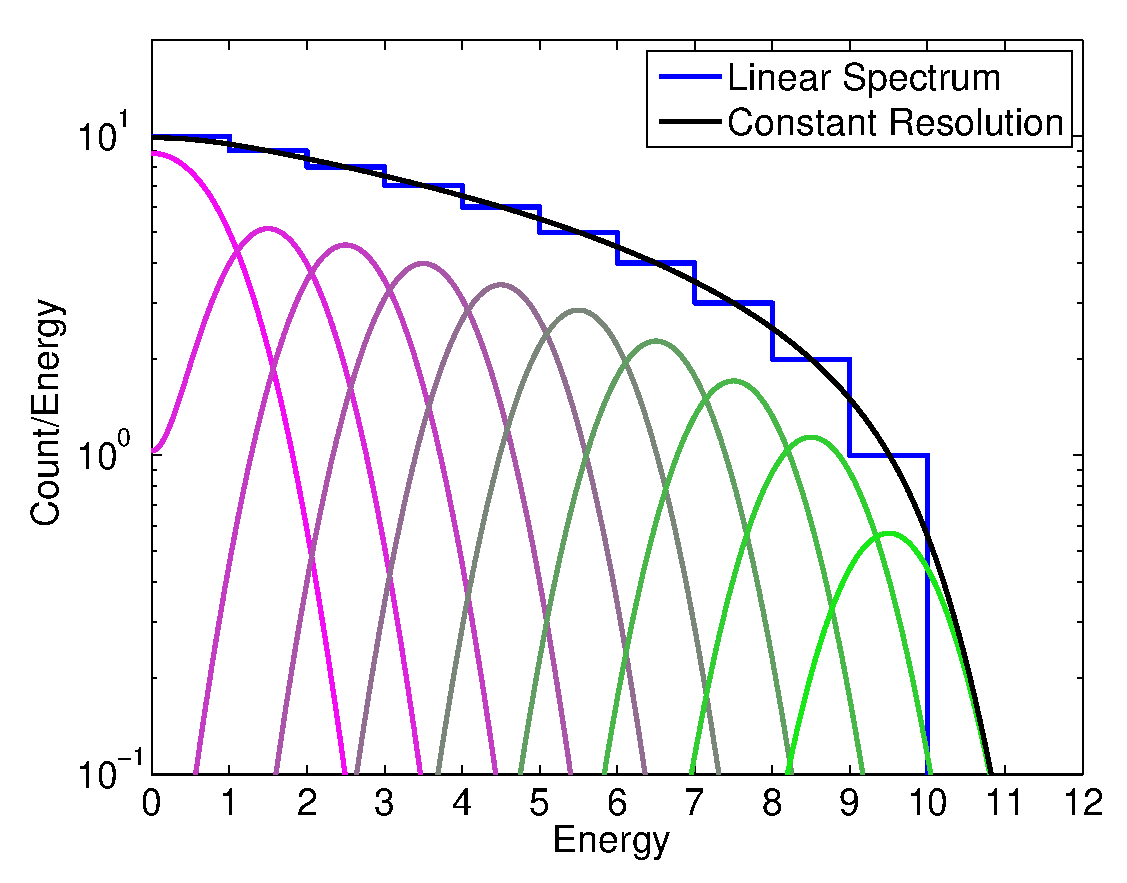
\includegraphics[width=70mm]{Chapter_Flucs/Figures/Toy_Model_lin_const}
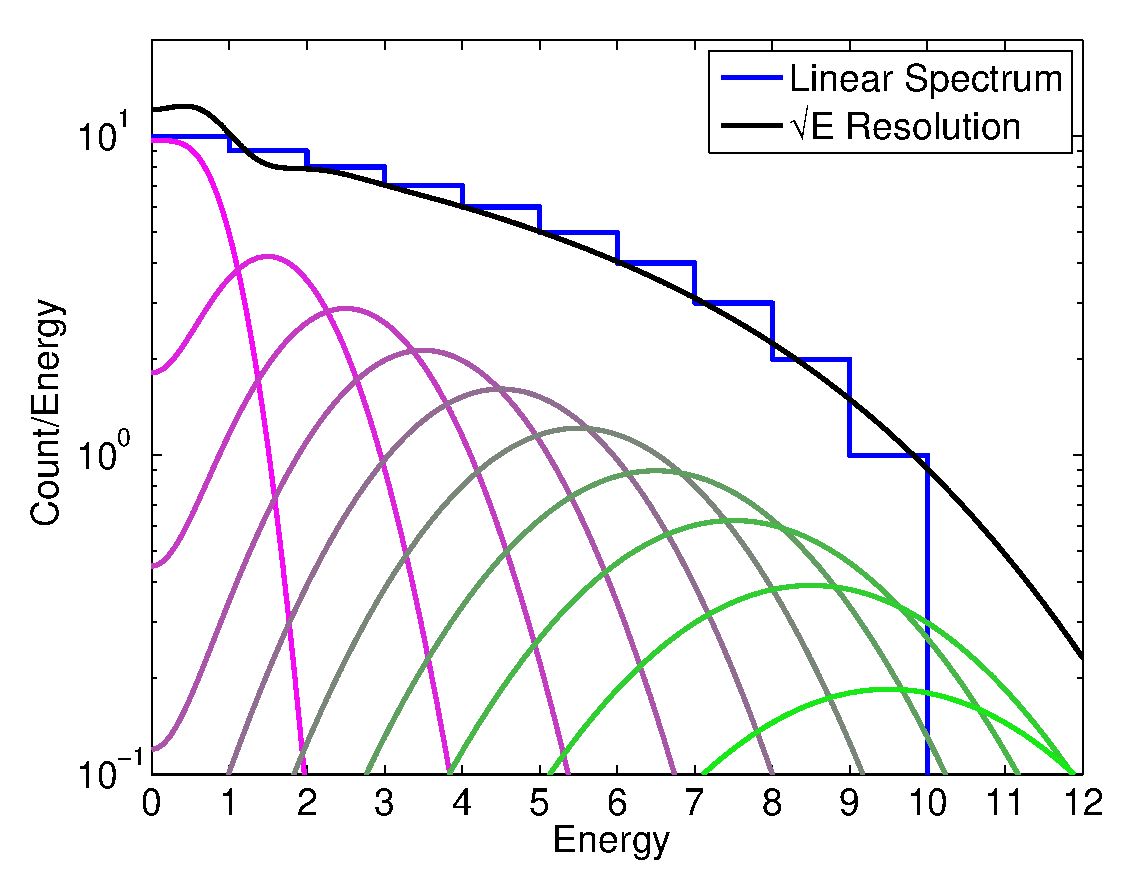
\includegraphics[width=70mm]{Chapter_Flucs/Figures/Toy_Model_lin_dep}
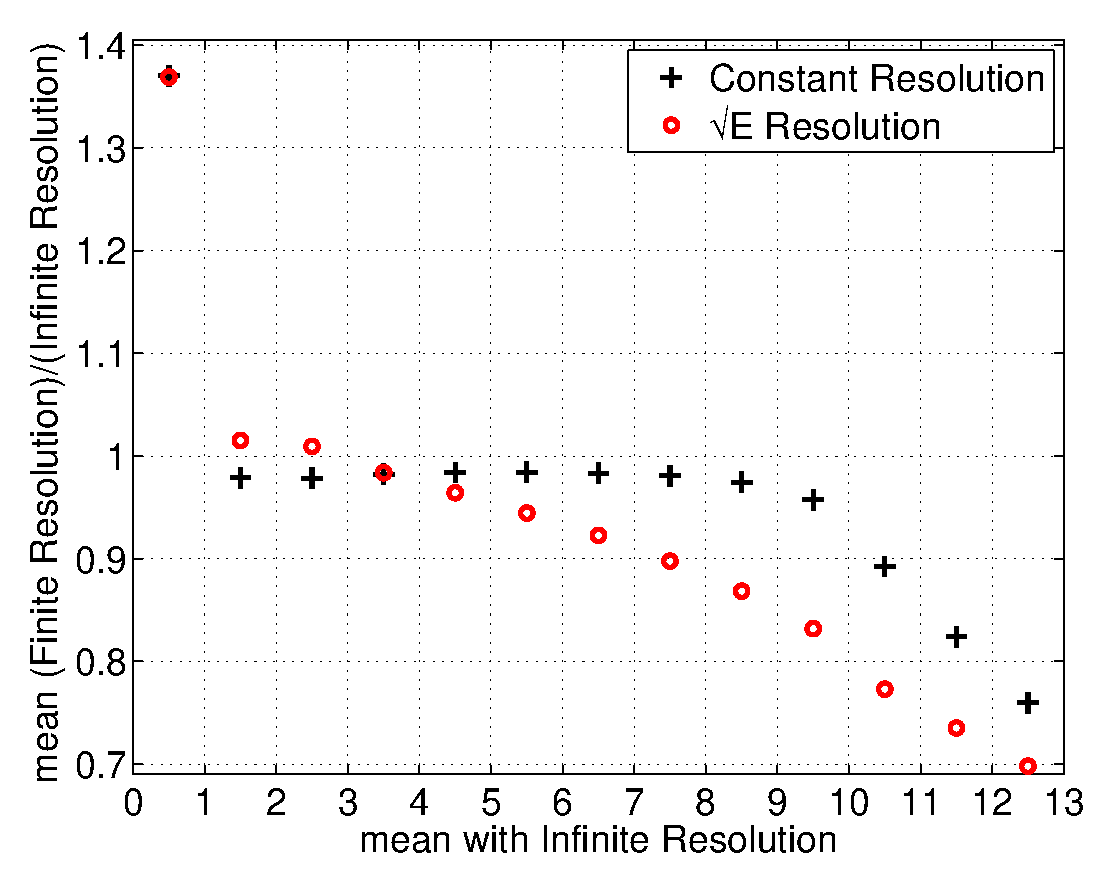
\includegraphics[width=70mm]{Chapter_Flucs/Figures/Toy_Model_mean_shift}
\caption{Top Left: A linearly decaying spectrum, in blue. The black curve represents the sum of the Gaussians assuming a constant resolution. Top Right: A linearly decaying spectrum, in blue. The black curve represents the sum of the Gaussians with a $\rm \sqrt{E}$ dependent resolution. Bottom: The observed mean, with finite resolution, compared to the real mean with infinite resolution. The black points are for the case with linear resolution and the red points represent the case with $\rm \sqrt{E}$ dependent resolution.}
\label{fig:Toy_Linear}
\end{figure}

\newpage


\section{Extracting Recombination Fluctuations from Tritium Calibration Data}

In this section we apply the methods outlined in this chapter and use them to extract the recombination fluctuations vs. energy from the tritium data. The first step in this process was calibrate the energy scale solving for g1 and g2 as outlined in \ref{Ch:E_Scale_Cal}. Second, the S1 and S2 signals of the tritium calibration data were corrected for spectral shape as outlined previously in section \ref{sec:Smear} and discussed in more detail in \ref{Ch:LYQY}. Finally, having modeled and measured the statistical and instrumented variances for light collection of the LUX detector \ref{eq:SigDet} \ref{eq:SigStat} \ref{eq:SigInst} the component of detector resolution in each energy bin can be calculated$\rm \chi_{Det}^2$ \ref{eq:SigCE}, ref{eq:Angle}, {eq:Centroid}. For the remained of the thesis we will work in centroid subtracted space as detailed in equation {eq:Centroid}, the results are identical to working in non centroid subtracted space using a bin width correction of equation \ref{eq:SigR_CE_lim}, which is the equivalent of making a linear approximation to the local slope.  


Since the tritium beta spectrum is continuous the calibration data is divided into energy bins. In each energy bin the mean of S1 and $\rm S2_b$ is measured and converted to the mean number of photons and electrons using g1 and g2. Once that is known the variance from detector resolution in each bin can be determined, defined as $\rm \chi_{Det}^2$ \ref{eq:Centroid}, \ref{eq:SigCE}. We then measure the variance of both the fluctuations in the photon and electron channels using Gaussian fits to the distributions in each energy bin, defined as $\rm \chi^2$. The recombination variance and variance from detector resolution are two independent processes making the observed variance in each bin $\rm \chi^2$ a sum of $\rm \chi_{Det}^2$ and $\rm \sigma_R^2$. We measure the variance of both the light and channel $\rm \chi_{\gamma}^2$ and $\rm \chi_e^2$ and solve for $\rm \sigma_{R_\gamma}^2$ and $\rm \sigma_{R_e}^2$ where the subscripts $\rm \gamma$ and e denote the photon and electron channel respectively. Using this we find
\begin{equation}
\rm \sigma_R^2 = \sigma_{R_\gamma}^2 = \sigma_{R_e}^2 = \chi^2-\chi_{Det}^2
\end{equation}
\noindent the same result as outlined in \ref{eq:SigR_Cent}. The recombination fluctuation $\rm \sigma R$ can be extracted from the tritium calibration data. The result of the tritium calibration is shown in figure \ref{fig:R_Flucs_Quanta} for both the 170 V/cm and 100 V/cm data. The 170 V/cm data had 140,000 tritium beta decays in the fiducial volume and the 100 V/cm data contained 4,500 events. 

\renewcommand{\baselinestretch}{1}
\small\normalsize
\begin{figure}[h!]\centering
 
\subcaptionbox{$\rm \sigma_R$, 170 V/cm \label{fig:5a}}{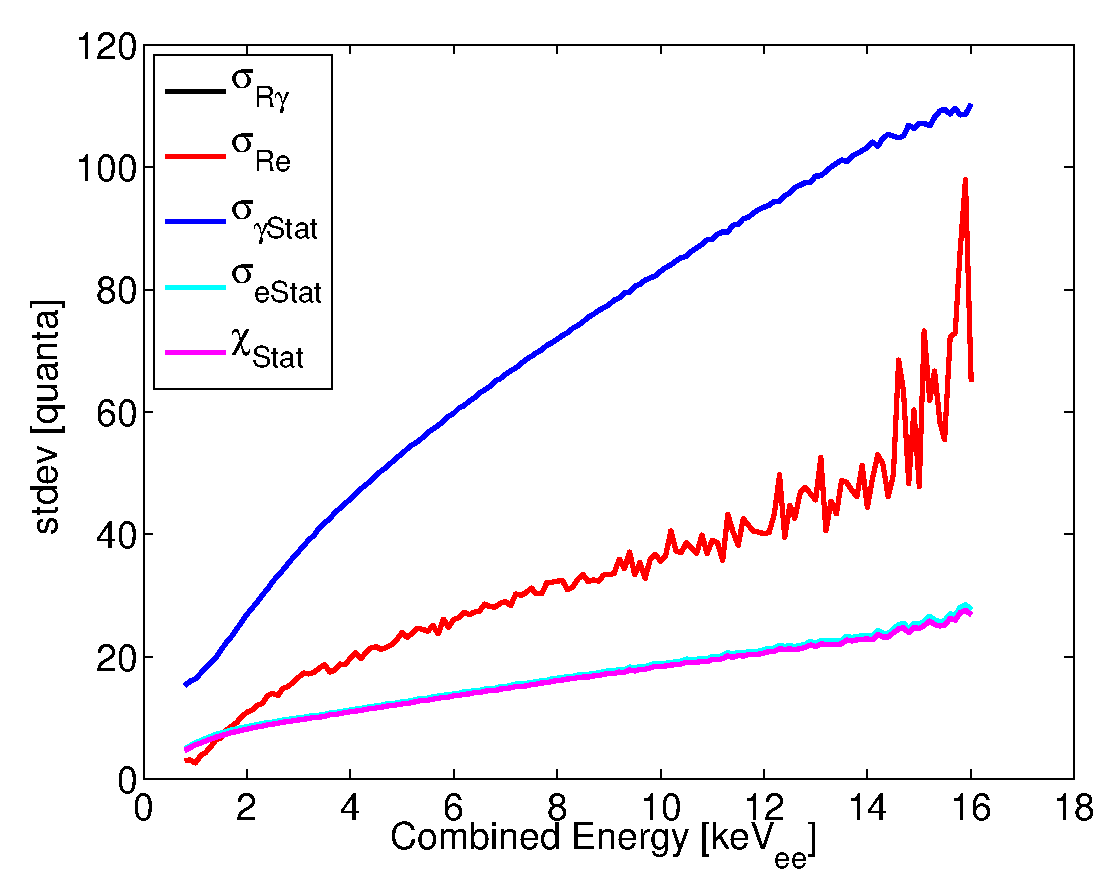
\includegraphics[width=75mm]{Chapter_Flucs/Figures/Iter1/std_fig_iter1LY_QY_iter1.eps}}
\hfill
\subcaptionbox{Quanta, 170 V/cm \label{fig:5b}}{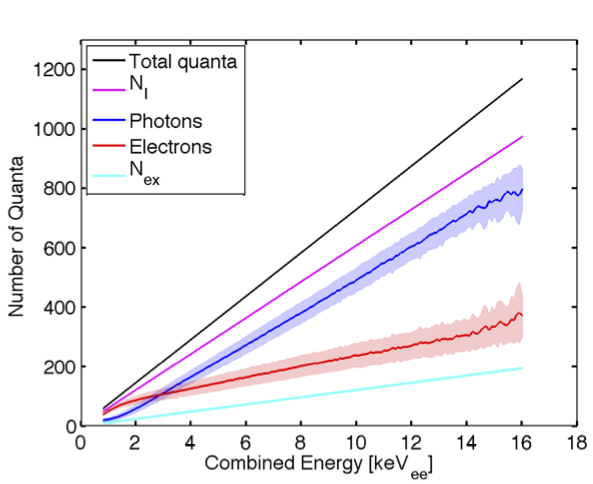
\includegraphics[width=73mm]{Chapter_Flucs/Figures/Iter1/quanta_inter1Tritium_LY_QY_iter1.png}}

\bigskip

\subcaptionbox{$\rm \sigma_R$, 100 V/cm \label{fig:5c}}{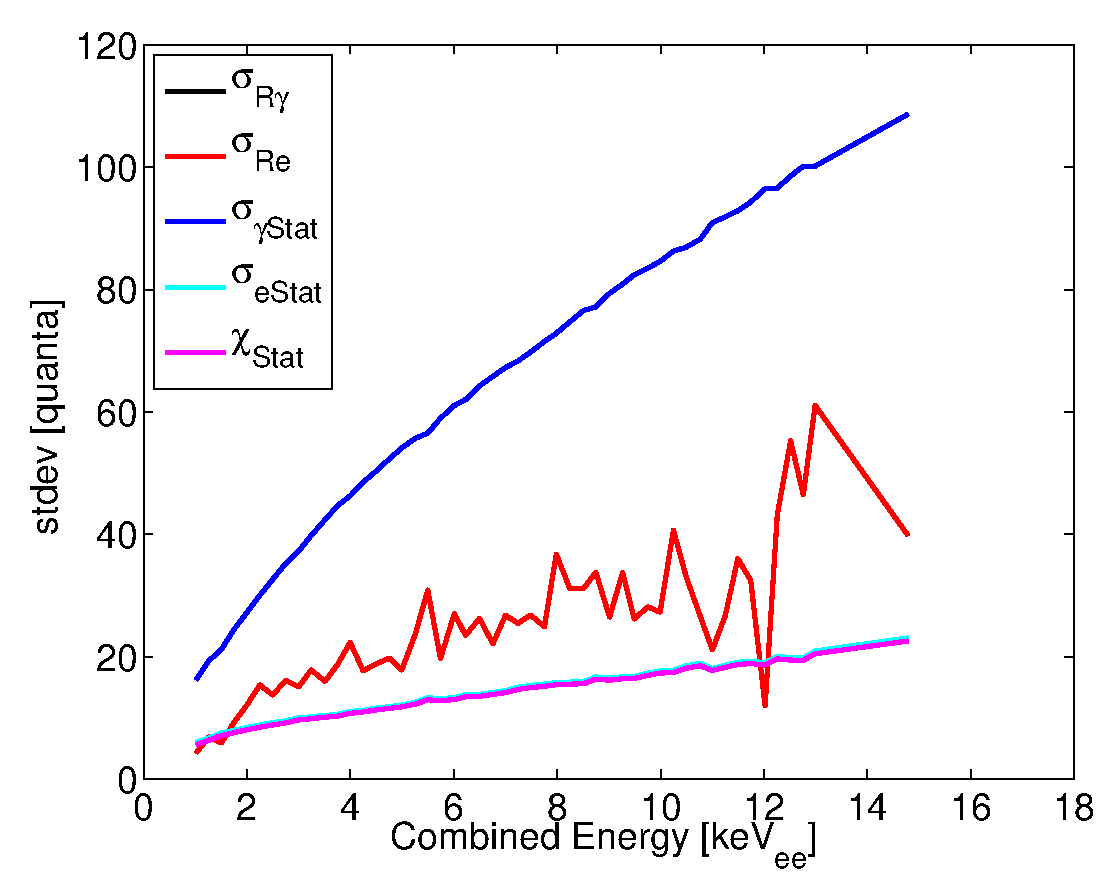
\includegraphics[width=75mm]{Chapter_Flucs/Figures/Iter1_100/std_fig_100_iter1Tritium_LY_QY_100_iter1.eps}}
\hfill
\subcaptionbox{Quanta, 100 V/cm \label{fig:5c}}{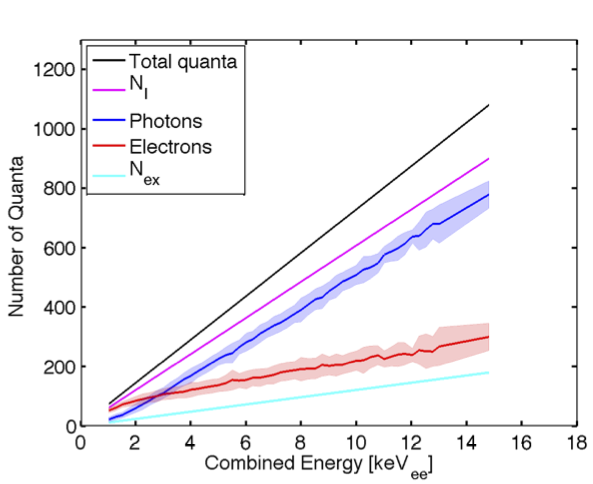
\includegraphics[width=73mm]{Chapter_Flucs/Figures/Iter1_100/quanta_100_iter1.png}}

 %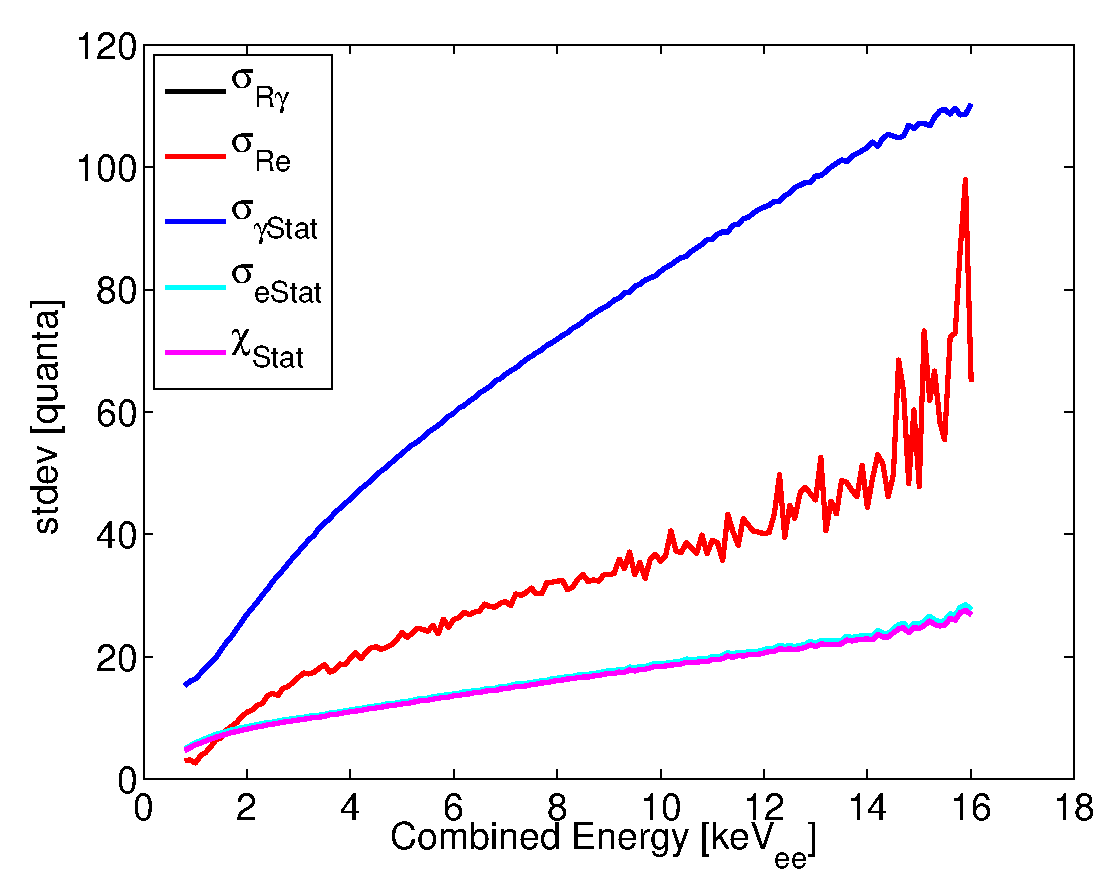
\includegraphics[width=100mm]{Chapter_Flucs/Figures/Iter1/std_fig_iter1LY_QY_iter1.eps}
 %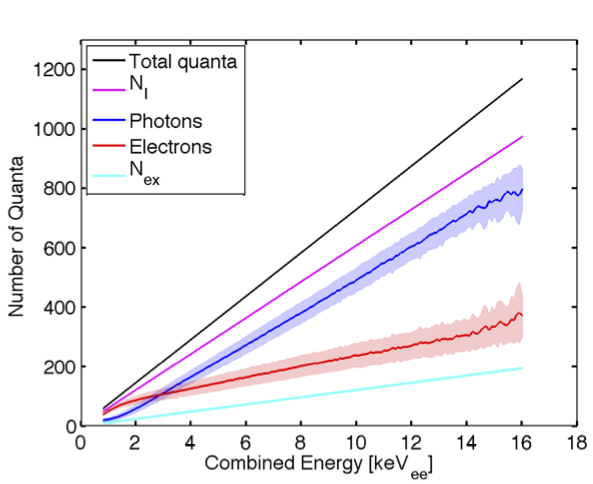
\includegraphics[width=100mm]{Chapter_Flucs/Figures/Iter1/quanta_inter1Tritium_LY_QY_iter1.png}
 %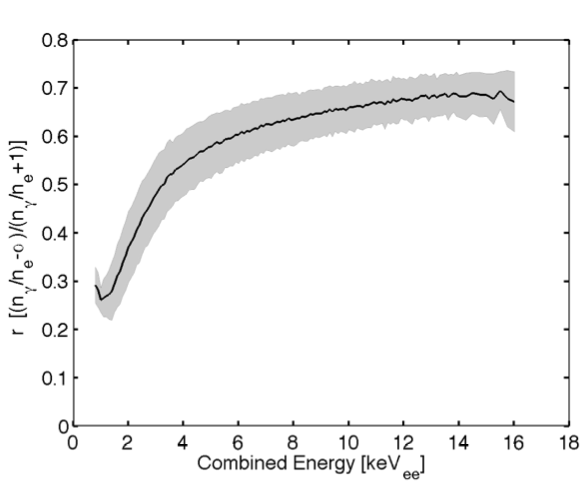
\includegraphics[width=70mm]{Chapter_Flucs/Figures/Iter1/R_iter1_LY_QY_iter1.png}
\caption{The figures on the left in \ref{fig:R_Flucs_Quanta} (a: 170 V/cm, c: 100 V/cm) show the extracted recombination fluctuation $\rm \sigma_R$ from the light (black) and change (red) channel denoted with subscript $\gamma$ and e respectively, note they are identical. Also shown are the fluctuations in light collection $\rm \chi_{\gamma_{Det}}^2$ (blue), charge collection $\rm \chi_{e_{Det}}^2$ (cyan), and their manifestation as detector resolution in a combined energy bin as $\rm \chi_{Det}$ (magenta). The figures on the right in in \ref{fig:R_Flucs_Quanta} (b: 170 V/cm, d: 100 V/cm) show the mean and one sigma standard deviation of the measured number of photons (blue) and electrons (red). Also shown is the total quanta (in black) which is the sum of photons and electrons and the expected number of ions (magenta) and excitons (cyan) using $\rm \alpha$ = 0.20.}
\label{fig:R_Flucs_Quanta}
\end{figure}
\renewcommand{\baselinestretch}{2}
\small\normalsize

The figures on the left in \ref{fig:R_Flucs_Quanta} (a: 170 V/cm, c: 100 V/cm)  show the extracted recombination fluctuation $\rm \sigma_R$ from the light (black) and change (red) channel denoted with subscript $\gamma$ and e respectively, note they are identical. Also shown are the fluctuations in light collection $\rm \chi_{\gamma_{Det}}^2$ (blue), charge collection $\rm \chi_{e_{Det}}^2$ (cyan), and their manifestation as detector resolution in a combined energy bin as $\rm \chi_{Det}$ (magenta). The detector resolution is actually slightly better than the resolution of the best channel, for the case of LUX is the charge collection. The remaining fluctuations in the light and charge channel after subtracting off the detector resolution in quadrature are shown in black and red, respectively. In regions where the measured recombinations are larger than the fluctuations caused by detector resolution any error in quanta counting from uncertainty on g1 and g2 is negligible as the signals add in quadrature. At the higher energy bins the uncertainty grows as the result becomes statistics limited. 

The figures on the left in \ref{fig:R_Flucs_Quanta} (a: 170 V/cm, c: 100 V/cm) show the extracted recombination fluctuation $\rm \sigma_R$ from the light (black) and change (red) channel denoted with subscript $\gamma$ and e respectively, note they are identical. Also shown are the fluctuations in light collection $\rm \chi_{\gamma_{Det}}^2$ (blue), charge collection $\rm \chi_{e_{Det}}^2$ (cyan), and their manifestation as detector resolution in a combined energy bin as $\rm \chi_{Det}$ (magenta).  The figures on the right in \ref{fig:R_Flucs_Quanta} (b: 170 V/cm, d: 100 V/cm) show the total quanta (black) which is the sum of the photons (blue) and electrons (red) and the expected number of ions (magenta) and excitons (cyan), using $\rm \alpha$ = 0.20. Since the detector resolution $\rm \chi_{Det}$ is solved for in terms of photons and electrons the means of the of number of photons and electrons in each energy bin must be measured first.


\subsection{Extracting Recombination fraction From Tritium Data}

Having measured the mean number of photons and electrons in each bin the value of recombination probability r can be determined using equation \ref{eq:Quanta}. Figure \ref{fig:R_T} shows the measurement of recombination probability r for the 170 V/cm and 100 V/cm tritium calibration data. The shaded region represents the one sigma of the recombination probability which can be thought of in terms of the recombination fluctuation $\rm \sigma_r = \sigma_R / n_{ions} $. Note, the bands converge below 4 $\rm keV_{ee}$ meaning that the light yields and charge yields also converge (discussed in ch 6), this leads to the energy thresholds at 1.5 keV being identical for at the two fields as seen in \ref{Ch:E_Scale_Cal}. Further, the ER and NR discrimination in this region overlap as will be discussed in the next subsection. All this translates into no observed improvement in either energy threshold or background rejection from 1 to 4 $\rm keV_{ee}$ between using a 100 and 170 V/cm field.

\begin{figure}[h!]\centering
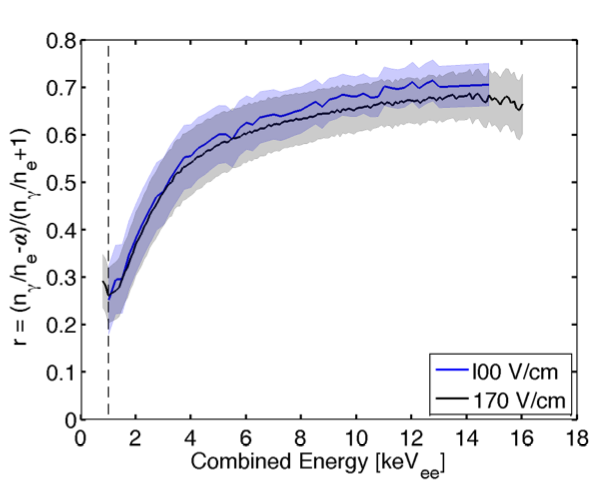
\includegraphics[width=120mm]{Chapter_Flucs/Figures/Iter1_100/R_comp.png}
\caption{Recombination Fraction at 170 V/cm (black) and 100 V/cm (blue). The shaded regions represent the one sigma of the observed fluctuations in recombination fractions $\rm \sigma_r$. The dashed line at 1.0 $\rm keV_{ee}$ represents the 50\% detection threshold.}
\label{fig:R_T}
\end{figure}


\subsection{Modeling the ER Band}

The main purpose of this section, and the tritium calibrations, are to be able to make predictions about WIMP sensitivity at various electric fields and in the WIMP search energies of interest, 1-5 $\rm keV_{ee}$. We now have the ability to reconstruct the electronic recoil band as it would appear with infinite detector resolution, with the ability to expand the band width by adding the measured detector resolution. Knowing the mean and width of the electronic recoil band and the mean of the NR band (described later) we can make predictions for ER and NR type discrimination which is a proxy for background event rejection.  

The mean of the ER band in discrimination space can be written as
\begin{equation}
\rm log_{10}(S2_b/S1) = log_{10} \left(\frac{(1-r)N_i}{(r+\alpha)N_i}\right) + log_{10}\left(\frac{g2}{g1}\right)
\label{eq:Band_Mean}
\end{equation}

\noindent where the observed charge and light signals $\rm S2_b$ and S1 have been converted to recombination probability r,  number of ions $\rm N_i$ and the exciton to ion ratio $\rm \alpha$ using equations \ref{eq:Gain} and \ref{eq:Quanta}.

The variance of the band can be written as,
\begin{equation}
\rm Var_{log_{10}(S2_b/S1)} = \frac{1}{\left(log(10)\right)^2} \times \sigma_R^2 \left( \frac{ - (\alpha+1) }{(1-r)(r+\alpha)N_i} \right)^2
\label{eq:Band_Var}
\end{equation}

\noindent Which has been written in terms of the number of ions $\rm N_i$, the recombination fraction r, and the measured recombination fluctuation $\rm \sigma_R$, defined to be $\rm \sigma_r\times N_i$. The result of the ER band's mean population and its corresponding 1 sigma fluctuation are shows in figure \ref{fig:ER_Band_Calc} for the case of 100 V/cm (blue) and 170 V/cm (black). This result shows the ER band with recombination fluctuations only. One can add light and charge collection fluctuations in quadrature to complete the modeling specific to any detector. Above 4 $\rm keV_{ee}$ the band separate as the higher drift field increased the charge extraction leading to better discrimination.

\begin{figure}[h!]\centering
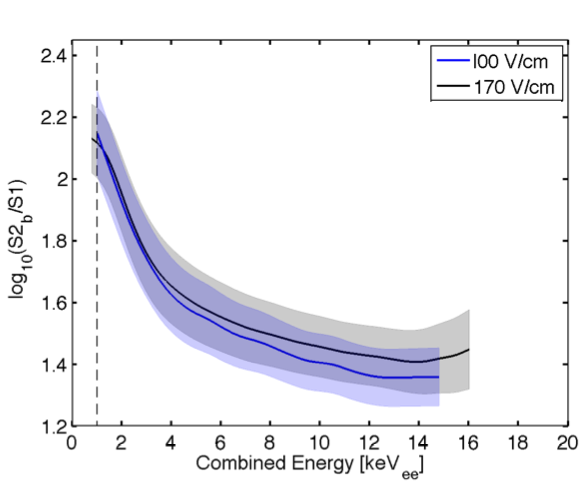
\includegraphics[width=130mm]{Chapter_Flucs/Figures/Iter1_100/Band_comp.png}
\caption{The result of the ER band's mean population and its corresponding 1 sigma fluctuation for the case of 100 V/cm (blue) and 170 V/cm (black). We find an over lap below 4 $\rm keV_{ee}$ where the additional strength of the drift field is hither improving threshold of discrimination. Above 4 $\rm keV_{ee}$ the band separate as the higher drift field increased the charge extraction leading to better discrimination.}
\label{fig:ER_Band_Calc}
\end{figure}

\newpage

\subsection{Measuring Alpha From the Tritium Data}

Having measured r and $\rm \sigma_r$ from the tritium calibration data the constancy of the exciton to ion ratio $\rm \alpha$ can be checked by requiring that as the number of ions tends to one the recombination fluctuations tend to that of a binomial process. This is justified as a single ion-electron pair will either recombine or not with some recombination probability r having a binomial variance written as,
\begin{equation}
\rm BinoVar= (1-r)rN_i
\label{eq:Bino_Var}
\end{equation}

\noindent where r is the recombination probability and $\rm N_i$ is the number of ions which can be thought of as the number of trials for the binomial process. In figure \ref{fig:Alpha_T} the y axis shows the ratio of the measured standard deviation of recombination to the standard deviation of a purely binomial process. The figure on the right has the expected binomial standard deviation on the x axis. The best alpha is one in which the observed standard deviation converges with that of a binomial process as the binomial variance tends to 1. The figure on the left has the number of ions available for recombination on the x axis. As the number of ions approaches one the standard deviation of recombination should become that of a binomial process. A single ion will either recombine or not with probability r.  The extrapolation is made by fitting the lowest energy bins above 90\% threshold 1.2 to 3 keV. We find that the best intercept converging to a purely binomial process is with $\alpha$ = 0.20 consistent with the measurement in \cite{Doke_alpha} and not 0.06 as used in \cite{Dahl_Thesis}.

\renewcommand{\baselinestretch}{1}
\small\normalsize
\begin{figure}[h!]\centering
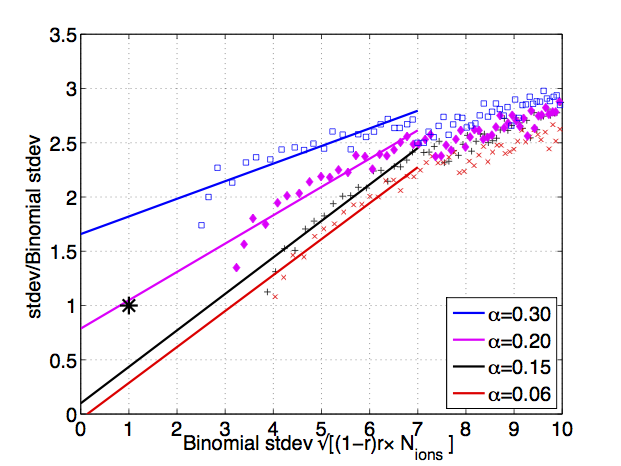
\includegraphics[width=74mm]{Chapter_Flucs/Figures/alpha/bino_norm_amp_iter1Tritium_LY_QY_100_iter1.png}
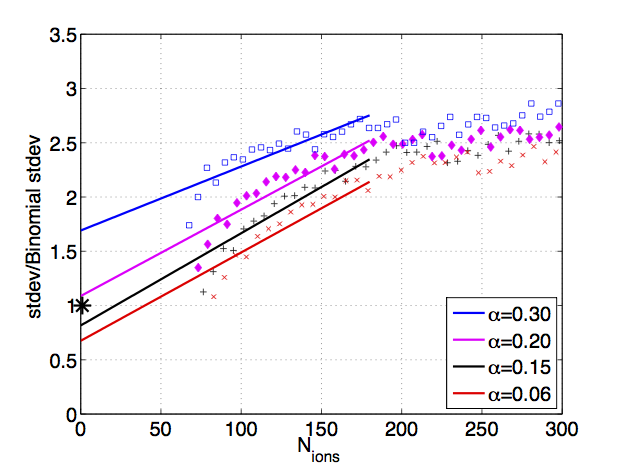
\includegraphics[width=74mm]{Chapter_Flucs/Figures/alpha/bino_norm_amp_ions_iter1Tritium_LY_QY_100_iter1.png}
\caption{Determining the best $\rm \alpha$ using the tritium calibration data, with $\rm \alpha$ = 0.3(blue), 0.2(magenta), 0.15(black) and 0.06(red). Left: The y axis is the ratio of the observed standard deviation of recombination to that of a binomial processes plotted vs. the expected binomial standard deviation on the x axis. The best $\rm \alpha$ is one in which the observed standard deviation converges with that of a binomial process as the binomial variance tends to 1. Right, the same y axis as on the left but plotted vs. the number of ions available for recombination. As the number of ions approaches one the standard deviation of recombination should become that of a binomial process. A single ion will either recombine or not with probability r.  The best intercept converging to a purely binomial process (black star) is with $\rm \alpha$ = 0.20. Note, the fits use only data above 90\% threshold at 1.2 keV, starting from the third data point from the left. The higher end cut off at  3 keV corresponds to the end of the fitted lines. }
\label{fig:Alpha_T}
\end{figure}
\renewcommand{\baselinestretch}{2}
\small\normalsize

\newpage

\section{Extracting Recombination Fluctuations from $\rm ^{137}Cs$ Calibration}

To expand the picture of recombination fluctuation to higher energies the same method used for the tritium calibration was applied to the Compton edge of a $\rm ^{137}Cs$ external calibration source. The $\rm ^{137}Cs$ source provides ER calibration data from the backscatter peak around 150 keV to the photo peak at 662 keV. Figure \ref{fig:Cs_LYQYR} on the left shows the measured mean number of photons, electron in each energy bin along with their one sigma fluctuation (shaded). The number of excitons and ions are also show assuming an $\alpha$ = 0.20. Once the mean number of photons and electrons are measured the recombination probability is determined and plotted on the right in figure \ref{fig:Cs_LYQYR}. The inflection around 662 keV is due to the sharp rise and fall of the photo peak skewing the measurement of number of photons and electrons.

\begin{figure}[h!]\centering
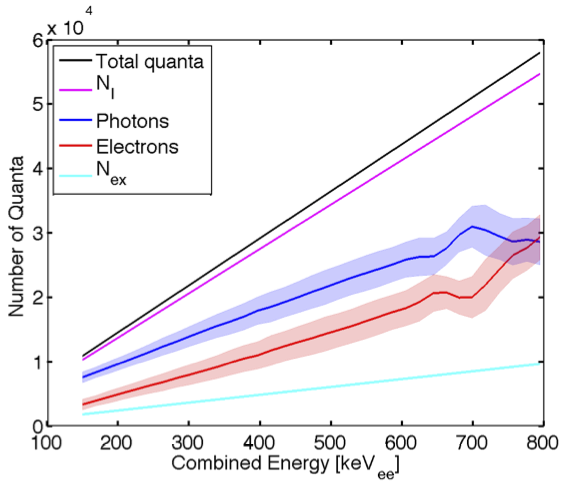
\includegraphics[width=72mm]{Chapter_Flucs/Figures/Cs/quanta_cs_.png}
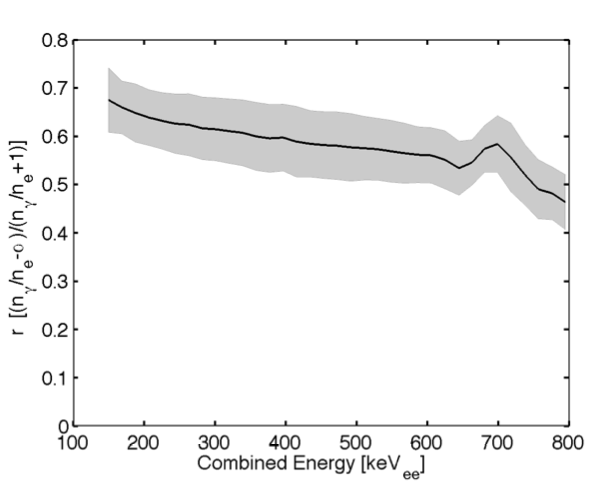
\includegraphics[width=72mm]{Chapter_Flucs/Figures/Cs/R_cs_.png}
\caption{ Left: The mean and one sigma standard deviation of the measured number of photons (blue) and electrons (red). Also shown is the total quanta (in black) which is the sum of photons and electrons and the expected number of ions (magenta) and excitons (cyan) using $\rm \alpha$ = 0.20. Right: The recombination probability r (solid black) and the one sigma fluctuation $\rm \sigma_{r}$ (shaded). }
\label{fig:Cs_LYQYR}
\end{figure}


\section{Recombination Fluctuations, The Bigger Picture}
We have now measured the recombination probability and fluctuation over a wide range of energies and at two fields for tritium (100 and 170 V/cm). The calibrations range from the 1.0 keV 50\% threshold with tritium to about 700 keV with the $\rm^{137}Cs$ calibration, and include the line sources used for the energy calibration in \ref{Ch:E_Scale_Cal} and table \ref{table:Cal_lines}. Also shown is a $\rm ^{57}Co$ calibration at a variety of electric fields ranging from 60 to 5000 V/cm from \cite{Dahl_Thesis}. Figure \ref{fig:R_Big} on the left shows the observed recombination fluctuation $\rm \sigma_R$ measurements vs. the standard deviation expected from a purely binomial process (equation \ref{eq:Bino_Var}). At our field of 100 and 170 V/cm we find good agreement with a simple power law fit which can be thought of as the fluctuation receiving an amplification over the underlying binomial process.

 Figure \ref{fig:R_Big} on the right shows the measured recombination fluctuation $\rm \sigma_R$ vs. the number of ions available for recombination $\rm N_i$. The x axis is chosen to be number of ions as recombination fluctuations only act on ions and not excitons, the conversion to energy on the x axis is simply $\rm E = W\times n_i (1 + \alpha ) $. It is found that the measured recombination fluctuation can be well described by a generic power law fit.

\begin{figure}[h!]\centering
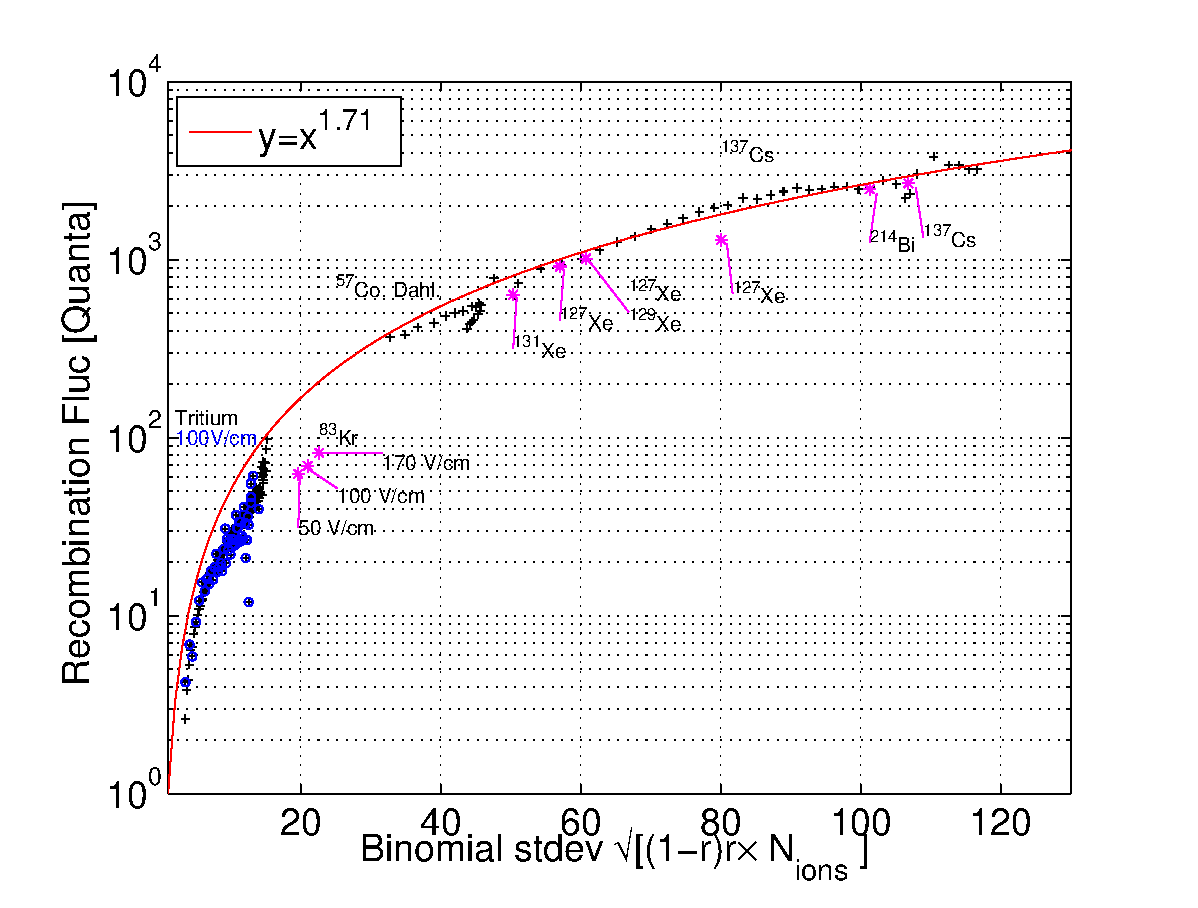
\includegraphics[width=73mm]{Chapter_Flucs/Figures/alpha/bino_amp_100_iter1.eps}
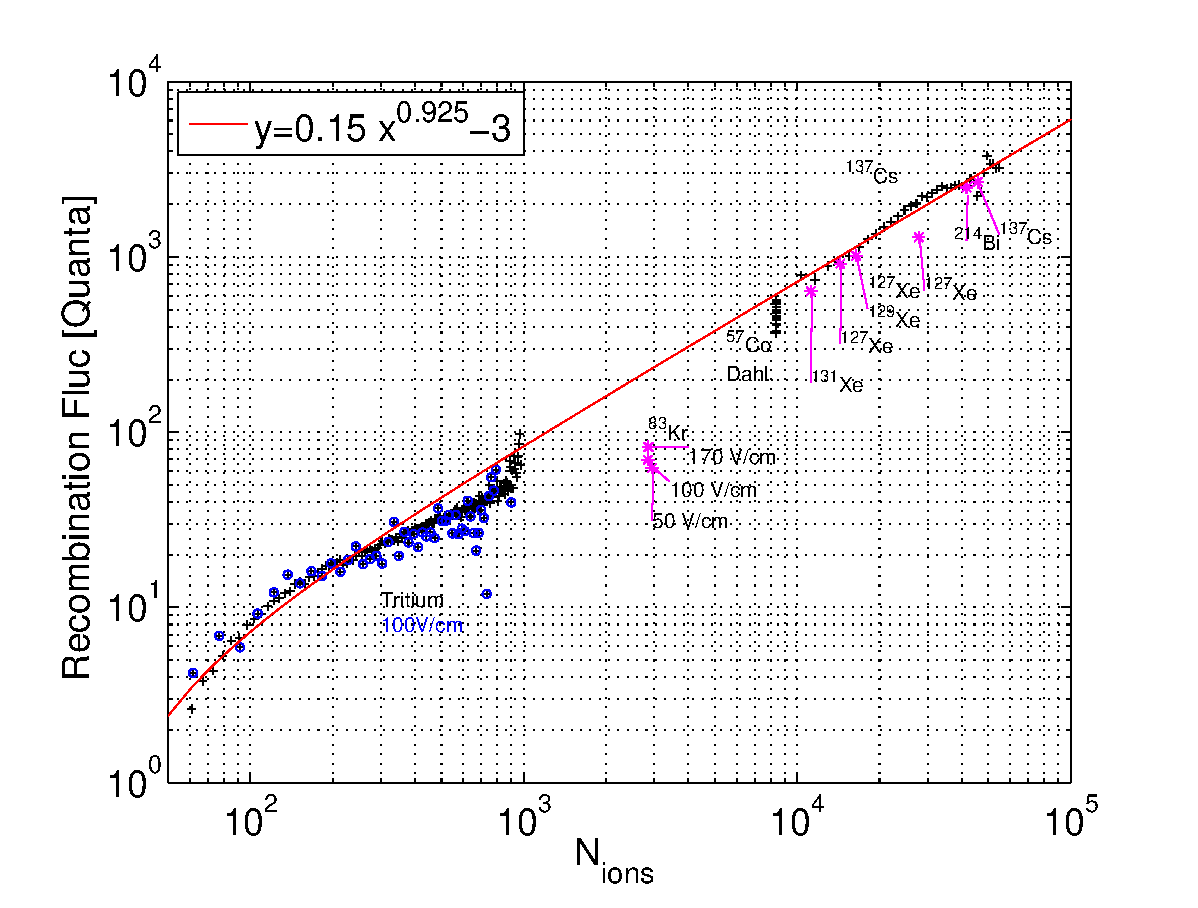
\includegraphics[width=73mm]{Chapter_Flucs/Figures/alpha/R_v_Ni_100_iter1.eps}
\caption{ Recombination fluctuations measurements are labeled on the plot and include data from tritium at 170 V/cm, tritium at 100 V/cm, $\rm ^{137}Cs$ calibration, the line sources used for the energy scale calibration listed in table \ref{table:Cal_lines} and a $\rm ^{57}Co$ calibration at a variety of electric fields ranging from 60 to 5000 V/cm from \cite{Dahl_Thesis}. Left: the observed recombination fluctuation $\rm \sigma_R$ measurements vs. the standard deviation expected from a purely binomial process,equation \ref{eq:Bino_Var}. }
\label{fig:R_Big}
\end{figure}


There have been numerous steps in this section culminating in expanding our knowledge by extracting as much information as possible from the tritium calibration source. We have measured that the best exciton to ion ratio $\rm \alpha$ measured to be 0.20 in the WIMP search energies, which is consistent with the measurement from \cite{Doke_alpha}. The value of alpha was constrained by extrapolating the recombination fluctuations from the tritium data from 3 to 1.2 keV and requiring that for a single ion-electron pair the fluctuation be purely binomial, shown in figure \ref{fig:Alpha_T}.

Most importantly, the measurements in this section can be used to predict the ER band in any xenon detector, as shown in figure \ref{fig:ER_Band_Calc}. The most critical results are those specific to our WIMP search, 10-100 GeV WIMPs, which are focused in the range of 1 to 5 $\rm keV_{ee}$ and well covered by the tritium calibration data. Having extracted the values of r and $\rm \sigma_r$ for ER events the generic mean and band widths can be determined. Thus, the ER band shape can be determined for any xenon detector with the application of the additional variance from the specific detector resolution. The knowledge of this band shape can be used to make predictions about the background rejection power of a given experiment. 

It is surprising to find that changing the drift filed from 100 V/cm to 170 V/cm had only an epsilon impact on the mean of ER band below 4 $\rm keV_{ee}$, figure \ref{fig:ER_Band_Calc}. Further, there was no impact on the energy threshold since the light and charge yields merge at the threshold of 1 keV. A more dramatic field dependance was expected from \cite{Dahl_Thesis} and \cite{NEST_2013}. However, the low energy region never been probed to such high precision as with the tritium calibration using the LUX detector. To expand upon the modeling at low energies it will be useful for the next science run using the LUX detector to take tritium calibration data at a verity of fields. This will allow us to predict exactly how much additional NR and ER discrimination can be achieved by increasing the field. %We also want to explore if the recombination fluctuation can truly be thought of an an amplification of the variance over that of the underlying binomial process of electron-ion pair recombination.
